%% ============================================================
%%  AI PROJECT REPORT – Group 2
%%  Plant Leaf Disease Detection
%%  Compile with: pdflatex (or xelatex) + bibtex/biber
%% ===========================================================
\documentclass[10pt, conference]{IEEEtran}

%% ── Packages ─────────────────────────────────────────────────
\usepackage[T1]{fontenc}
\usepackage[utf8]{inputenc}
\usepackage[english]{babel}
\usepackage{lmodern}
\usepackage{microtype}

\usepackage{amsmath, amssymb, amsfonts}
\usepackage{mathtools}

\usepackage{graphicx}
\usepackage{booktabs}
\usepackage{multirow}
\usepackage{array}
\usepackage{balance}
\usepackage[table,xcdraw]{xcolor}

\usepackage{hyperref}
\hypersetup{hidelinks}

\usepackage{url}

%% ── Colour helpers ───────────────────────────────────────────
\definecolor{bestred}{RGB}{180,0,0}
\definecolor{secondblack}{RGB}{0,0,0}

%% ============================================================
\begin{document}

\title{Plant Leaf Disease Detection}

\author{
    \IEEEauthorblockN{Hoang Bao Long, Nguyen Thanh Luan, Dang Vu Lan, Pham Trung Kien, Nguyen Dinh Khoi}
    \IEEEauthorblockA{Introduction to Artificial Intelligence, Group 2}
}

\maketitle

\begin{abstract}
Automated plant leaf disease recognition can support timely crop management, but practical systems must balance predictive performance with computational cost. Models that perform well on curated laboratory images may also be substantially less effective on visually complex field data. This study therefore benchmarks lightweight approaches for both disease classification and lesion detection rather than proposing a new architecture. We compare an Advanced Depthwise Separable CNN and V2PlantNet for classification, together with YOLO-LeafNet variants and standard YOLO baselines for detection. The models are trained and evaluated separately on PlantVillage, which contains controlled-background images, and PlantDoc, which contains field-collected images with clutter, occlusion, and illumination variation. Evaluation covers accuracy, precision, recall, F1-score, mean Average Precision, parameter count, and inference latency. On PlantVillage, classification accuracy exceeds 98\% and detection mAP@50 exceeds 99\%. On PlantDoc, the best classification accuracy is 53.96\%, while YOLOv12s obtains the highest detection mAP@50 of 63.65\%. V2PlantNet uses approximately 0.38 million parameters and reaches 8.69 ms classification latency on PlantDoc. These results quantify a substantial laboratory-to-field performance gap and identify practical accuracy--efficiency trade-offs. The selected detector is also demonstrated in a desktop application that visualizes detections, reports confidence, and generates Vietnamese diagnostic guidance through a large language model.
\end{abstract}

\begin{IEEEkeywords}
    Plant disease recognition, lightweight deep learning, image classification, object detection, field imagery.
\end{IEEEkeywords}

\section{Introduction}
\label{sec:intro}

Plant diseases threaten crop productivity, food quality, and farm income, making timely diagnosis an important component of sustainable agriculture. Manual visual inspection remains common but is labor-intensive, difficult to scale, and dependent on specialist experience. Computer-vision systems can support this process by consistently classifying visible symptoms and localising diseased regions in leaf images~\cite{harakannanavar2022,zhao2025,salka2025}. Their practical value is especially relevant where repeated field inspection or access to plant pathologists is limited.

Recent research has progressed from conventional machine-learning pipelines to convolutional neural networks (CNNs) and one-stage detectors. Advanced depthwise CNNs combine separable convolution, attention, and residual connections to reduce computation~\cite{ashurov2025}; V2PlantNet adapts MobileNet for compact multi-class recognition~\cite{nnamdi2025}; and YOLO-LeafNet targets multi-species disease localisation~\cite{kaur2025}. These studies continue a broader trend toward efficient agricultural vision models~\cite{sujatha2025}. Nevertheless, results obtained on controlled-background datasets such as PlantVillage are not directly indicative of performance on field images containing clutter, occlusion, scale variation, and uneven illumination.

This work does not claim to fill an unaddressed architectural gap. Instead, it continues the benchmarking tradition and raises a practical question: how do representative lightweight classification and detection models compare, in both predictive quality and efficiency, when evaluated in controlled and field-oriented data settings? Answering this question is useful for model selection even when the underlying architectures have been published previously.

To investigate this question, we implement an Advanced Depthwise Separable CNN and V2PlantNet for classification, and evaluate YOLO-LeafNet variants and standard YOLO models for object detection. Experiments are conducted separately on PlantVillage and PlantDoc using task-appropriate metrics, parameter counts, and measured inference latency. Because the models are trained separately on each dataset, the comparison quantifies a dataset-dependent laboratory-to-field performance gap rather than a formal cross-domain generalisation experiment.

The principal findings are that all evaluated models perform strongly on PlantVillage, whereas performance is markedly lower on PlantDoc. The Advanced CNN reaches 53.96\% classification accuracy on PlantDoc, YOLOv12s reaches 63.65\% mAP@50, and V2PlantNet offers the smallest classification model and lowest measured PlantDoc latency. These results motivate cautious interpretation of laboratory benchmarks and deployment-oriented evaluation.

The primary contributions of this paper are summarized as follows:
\begin{enumerate}
    \item We design and implement an end-to-end evaluation pipeline comparing lightweight classification (Advanced DSC-CNN, V2PlantNet) and object detection (YOLO-LeafNet) models for plant leaf disease diagnostics.
    \item We benchmark these architectures using edge-ready metrics including parameter counts, inference latency, classification accuracy, and mean Average Precision (mAP).
    \item We quantify the performance difference between a controlled laboratory-style dataset (PlantVillage) and a noisy field-oriented dataset (PlantDoc), while explicitly distinguishing this comparison from cross-domain evaluation.
    \item We integrate the selected detector into a responsive desktop diagnostic application with bounding-box visualisation, confidence reporting, and LLM-assisted Vietnamese guidance.
\end{enumerate}

\begin{figure}[!t]
    \centering
    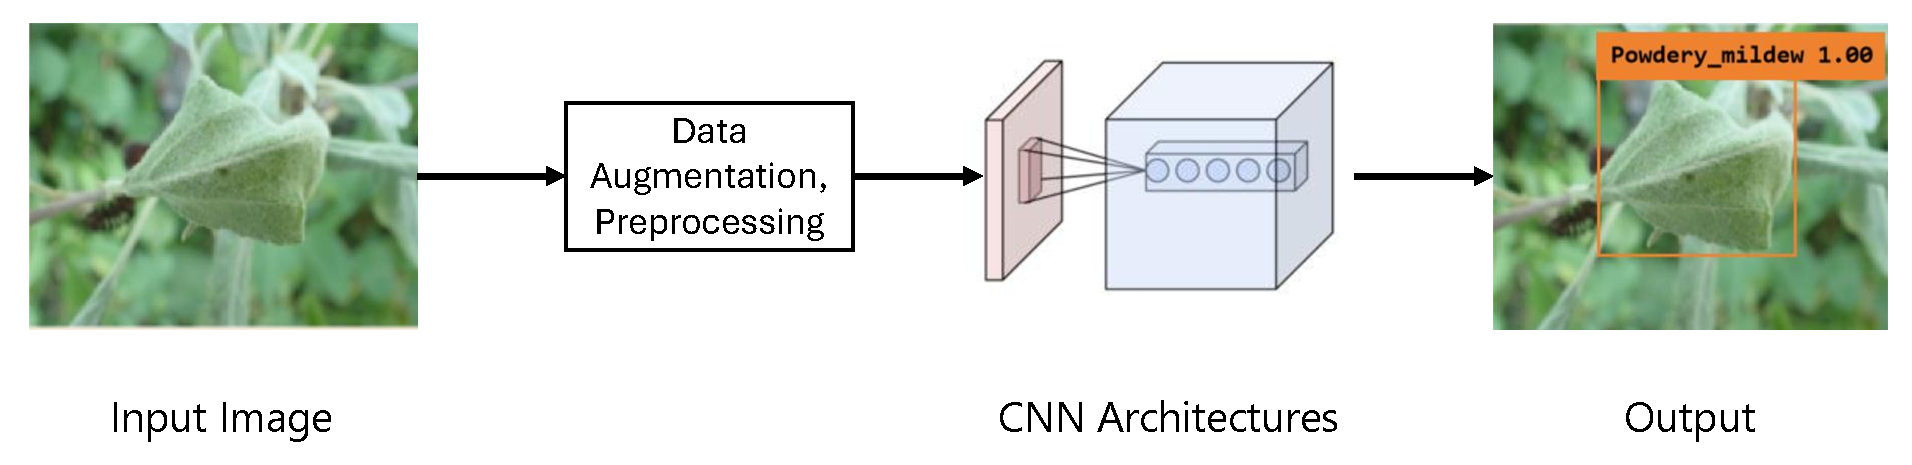
\includegraphics[width=0.9\linewidth]{figures/General_cropped.pdf}
    \caption{Overview of the Plant Leaf Disease Detection Pipeline.}
    \label{fig:pipeline_overview}
\end{figure}

\section{Related Works}
\label{sec:literature}

Deep learning-based plant disease detection and classification has seen significant progress, moving from laboratory-constrained classification pipelines to real-time, field-deployed object detection networks. Understanding this evolution requires analyzing both review-based taxonomies and specific hybrid methodologies.

Harakannanavar et al.~\cite{harakannanavar2022} and Salka et al.~\cite{salka2025} provide comprehensive reviews on convolutional neural network (CNN) architectures and traditional machine learning pipelines applied to agricultural diagnostics. They outline the typical visual processing flow, which commonly begins with preprocessing (e.g., resizing and contrast enhancement via Histogram Equalization) and K-means clustering segmentation to isolate diseased leaf regions or lesions. These segmented regions are then characterized using frequency-based or texture-based feature extractors like the Gray-Level Co-occurrence Matrix (GLCM), Discrete Wavelet Transform (DWT), and Principal Component Analysis (PCA) for dimensionality reduction. Finally, classifiers such as Support Vector Machines (SVM), k-Nearest Neighbors (k-NN), and deep CNN backbones are benchmarked. Their reviews show that while classical ML approaches are computationally simple, end-to-end CNN structures yield superior accuracies (exceeding 99\% on controlled datasets like PlantVillage) due to their automatic spatial feature representation learning.

Zhao et al.~\cite{zhao2025} offer an extensive review of plant leaf disease identification by structuring deep learning algorithms into three primary object detection classes:
\begin{enumerate}
    \item \textbf{Two-Stage Detection Networks}: Models such as Faster R-CNN and Mask R-CNN that first generate region proposals and then perform localized disease classification. Although highly precise for fine-grained lesions, their multi-stage nature results in significant computational latency.
    \item \textbf{One-Stage Detection Networks}: Real-time networks like SSD and the YOLO family (ranging from YOLOv3 to YOLOv12). These systems frame detection as a single regression task, optimizing inference latency for mobile or drone-based edge systems.
    \item \textbf{Anchor-Free Detection Networks}: Architectures such as CenterNet, CornerNet, and RT-DETR that identify symptoms by predicting keypoints (e.g., center points or corners) directly, improving robustness under heavy leaf occlusion and overlapping conditions.
\end{enumerate}

Complementing these architectures, Sujatha et al.~\cite{sujatha2025} investigate hybrid pipelines that combine deep visual feature extraction with classical machine learning classifiers. By using pre-trained CNN backbones (such as VGG19 and Inception v3) with their classification layers removed as feature vector generators, and feeding these vectors into traditional classifiers (SVM, RF, k-NN, AdaBoost, and Decision Trees), they demonstrate that optimal combinations are dataset-dependent. For instance, Inception v3 coupled with an SVM classifier performs best on banana and potato leaves, while VGG19 paired with k-NN is optimal for custard apple and fig leaves. Their work underlines the importance of matching feature representation styles with specific crop characteristics to optimize edge performance.

\section{Problem Formulation}
\label{sec:problem}

To establish a formal basis for evaluating lightweight diagnostics, we mathematically formulate the plant leaf disease detection problem as two distinct computer vision tasks—Classification and Object Detection—subject to edge-hardware computational constraints.

Let $\mathcal{X} \subset \mathbb{R}^{H \times W \times C}$ denote the input image space, representing plant leaf images of height $H$, width $W$, and $C$ color channels (typically $C=3$ for RGB color space). We define the set of known health and disease classes as $\mathcal{Y} = \{1, 2, \dots, K\}$, where $K$ is the total number of target categories across plant species and pathologies.

\subsection{Pathology Classification Task}
The objective of the classification task is to learn a mapping function $f: \mathcal{X} \to [0, 1]^K$ that predicts the probability distribution over the pathology classes for a given leaf image $\mathbf{X} \in \mathcal{X}$. The predicted class distribution $\mathbf{\hat{y}} = f(\mathbf{X}; \mathbf{W}_{\text{cls}})$ is parameterized by the weights $\mathbf{W}_{\text{cls}}$ of the classification network. The network is trained by minimizing the cross-entropy loss function $\mathcal{L}_{\text{cls}}$ over a training dataset of $N$ samples, as expressed in (\ref{eq:cross_entropy}).
\begin{equation}
    \label{eq:cross_entropy}
    \mathcal{L}_{\text{cls}}(\mathbf{W}_{\text{cls}}) = -\frac{1}{N} \sum_{i=1}^{N} \sum_{k=1}^{K} y_{i,k} \log \hat{y}_{i,k}
\end{equation}
where $y_{i,k} \in \{0, 1\}$ represents the ground-truth binary indicator for the $k$-th class of the $i$-th image.

\subsection{Pathology Detection and Localization Task}
For tasks requiring precise spatial localization of individual disease lesions on a leaf, the problem is formulated as object detection. The goal is to learn a mapping $g: \mathcal{X} \to \mathcal{B}$ that predicts a set of bounding boxes and associated class labels for an input image $\mathbf{X}$. The output space $\mathcal{B} = \{\mathbf{b}_1, \mathbf{b}_2, \dots, \mathbf{b}_M\}$ consists of $M$ detected lesions, where each box $\mathbf{b}_j$ is defined by the tuple presented in (\ref{eq:bbox_tuple}).
\begin{equation}
    \label{eq:bbox_tuple}
    \mathbf{b}_j = \left(c_j, x_j, y_j, w_j, h_j, p_j\right)
\end{equation}
where $c_j \in \mathcal{Y}$ is the predicted class label, $(x_j, y_j, w_j, h_j) \in [0, 1]^4$ are the normalized coordinates representing the bounding box center, width, and height, and $p_j \in [0, 1]$ is the confidence score of the detection. The detection network weights $\mathbf{W}_{\text{det}}$ are optimized by minimizing a multi-task loss combining localization and classification objectives, as formulated in (\ref{eq:detection_loss}).
\begin{equation}
    \label{eq:detection_loss}
    \mathcal{L}_{\text{det}}(\mathbf{W}_{\text{det}}) = \lambda_{\text{box}} \mathcal{L}_{\text{CIoU}}(\mathbf{W}_{\text{det}}) + \lambda_{\text{cls}} \mathcal{L}_{\text{BCE}}(\mathbf{W}_{\text{det}})
\end{equation}
where $\mathcal{L}_{\text{CIoU}}$ is the Complete Intersection over Union loss for bounding box regression, $\mathcal{L}_{\text{BCE}}$ is the Binary Cross-Entropy loss for category classification, and $\lambda_{\text{box}}$, $\lambda_{\text{cls}}$ are scaling factors.

\subsection{Lightweight Multi-Objective Optimization Constraint}
In edge-deployment scenarios, model selection cannot be guided solely by minimizing prediction losses. Instead, we formulate the model selection as a constrained multi-objective optimization problem. Let $\mathcal{M}$ represent the space of candidate models. We define the following metrics for any model $M \in \mathcal{M}$:
\begin{itemize}
    \item $P(M)$: The total number of trainable parameters (representing memory footprint).
    \item $F(M)$: The number of floating-point operations (FLOPs) required for inference.
    \item $L(M)$: The average inference latency (measured in milliseconds) on the target hardware.
    \item $A(M)$: The predictive capability, measured via classification accuracy $A_{\text{cls}}(M)$ or detection mean Average Precision $A_{\text{det}}(M)$.
\end{itemize}

The lightweight design goal is to find a model $M^*$ that optimizes the objective function given in (\ref{eq:optimization_objective}).
\begin{equation}
    \label{eq:optimization_objective}
    M^* = \arg\min_{M \in \mathcal{M}} \left[ P(M), L(M) \right]
\end{equation}
This optimization is subject to the constraint on predictive capability defined in (\ref{eq:optimization_constraint}).
\begin{equation}
    \label{eq:optimization_constraint}
    A(M^*) \ge \theta
\end{equation}
This formulation mathematically frames the trade-offs analyzed in this paper between accuracy, resource consumption, and inference speed.

%% ============================================================
\section{Method}
\label{sec:method}

This section describes the datasets used, the preprocessing and augmentation pipeline, and the lightweight deep learning model architectures evaluated in this project.

\subsection{Datasets}
\label{subsec:datasets}

To assess model performance, we use two benchmark datasets representing controlled-laboratory and unstructured real-world conditions. A visual comparison of samples is shown in Figure~\ref{fig:dataset_samples}.

\subsubsection{PlantVillage}
PlantVillage~\cite{hughes2015plantvillage} is a widely recognized benchmark for plant disease classification. It contains \textbf{54,305+ leaf images} spanning \textbf{14 plant species} (including Apple, Cherry, Corn, Grape, Peach, Potato, Strawberry, Tomato, etc.) and \textbf{38 distinct categories} comprising 26 disease states and 12 healthy states. The dataset's primary characteristics are high resolution and uniform, solid grey backgrounds. While these controlled settings simplify color and shape segmentation, they do not reflect actual agricultural environments, often leading to overly optimistic model metrics.

\subsubsection{PlantDoc}
PlantDoc~\cite{singh2020plantdoc} is a dataset designed to evaluate models under realistic field conditions. It contains \textbf{2,598 leaf images} representing \textbf{13 plant species} and \textbf{30 classes}. Unlike PlantVillage, the images in PlantDoc are collected in unstructured environments and contain severe clutter, occlusions, varying solar illumination, shadows, and camera blur. Annotations are provided as normalized bounding boxes for object detection, which we crop to generate samples for classification training.

\subsubsection{Taxonomy Mapping, Filtering, and Balancing}
To align the datasets for consistent evaluation, we implement a class mapping configuration (\texttt{PLANTDOC\_MAP}) to unify minor spelling and naming discrepancies in the folders into a standardized taxonomy (\texttt{UNIFIED\_CLASSES}). Furthermore, we apply an inter-dataset filter to exclude crop species that lack a complete representation of both healthy and diseased states across both sets, ensuring fair multi-crop disease discrimination.

For the classification task, the PlantDoc training split exhibits severe class imbalance. We address this by computing reciprocal class frequencies and utilizing a PyTorch \texttt{WeightedRandomSampler} within the DataLoader. This dynamically up-samples under-represented categories and down-weights majority classes, presenting a uniform class distribution (nominally $N_{\text{train}} = 1000$ instances per class) during training while keeping the validation and test sets purely composed of original, unaltered real images to prevent data leakage.

\begin{figure}[!t]
    \centering
    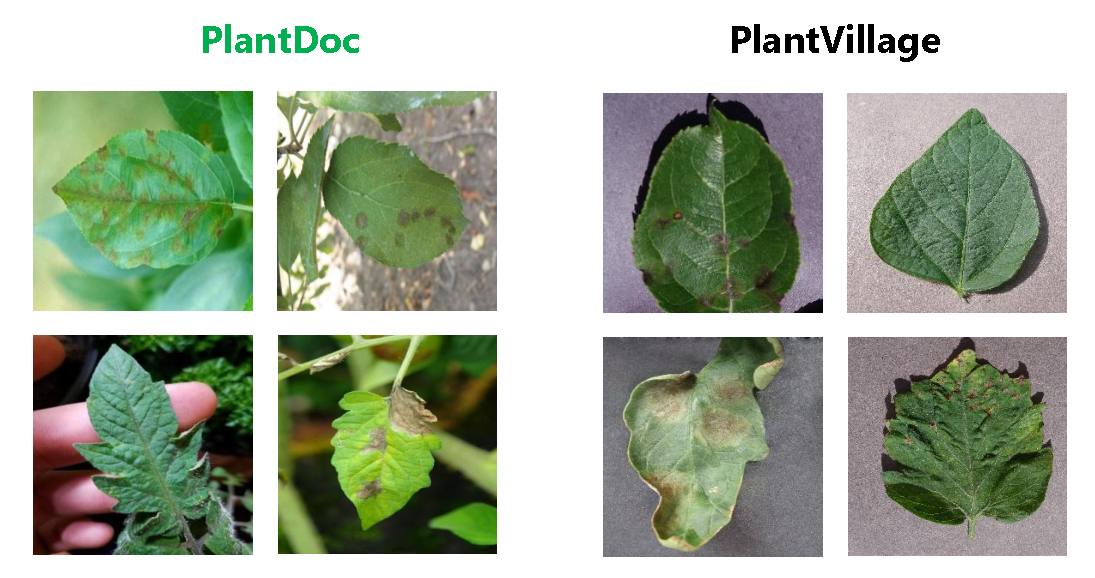
\includegraphics[width=0.85\linewidth]{figures/plantdoc_plantvillage.pdf}
    \caption{Sample images from PlantDoc (left) and PlantVillage (right).}
    \label{fig:dataset_samples}
\end{figure}

%% ============================================================
\subsection{Data Augmentation and Preprocessing}
\label{subsec:data}

\subsubsection{Classification Pipeline}
\label{subsec:data_classification}

The preprocessing pipeline for the classification task consists of four stages,
illustrated in Figure~\ref{fig:cls_pipeline}.

\begin{enumerate}
    \item \textbf{Raw Data.}
          Images are stored with original class labels
          (e.g.\ \texttt{Apple\_Scab}, \texttt{Tomato\_Healthy}).

    \item \textbf{Dataset Management.}
          Labels are standardised and image paths are catalogued.
          Corrupt or unreadable images are silently skipped via a fail-safe
          mechanism.

    \item \textbf{Preprocessing \& Sampling.}
          Augmentation transforms — Resize, Random Crop, and Colour Jitter —
          are applied to training images. All images are then normalised.
          A \texttt{WeightedRandomSampler} is applied to counteract class
          imbalance by assigning higher sampling weights to under-represented
          classes.

    \item \textbf{DataLoader \& Training.}
          Batches of images and labels are fed to the model.
\end{enumerate}

\begin{figure*}[t]
    \centering
    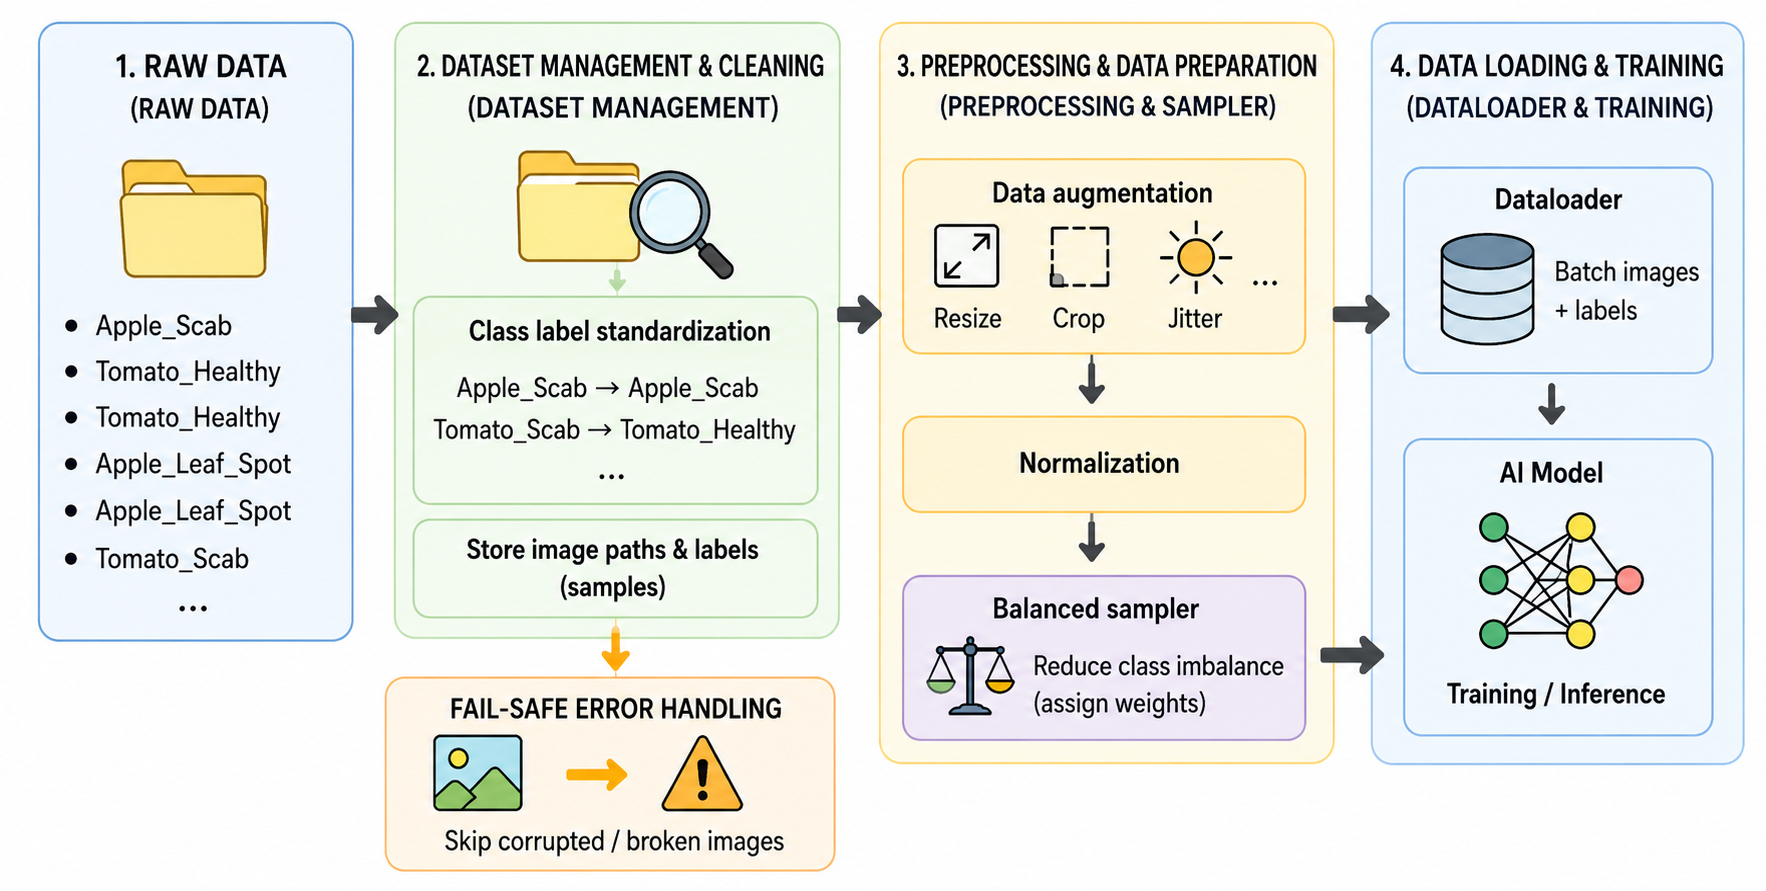
\includegraphics[width=0.85\linewidth]{figures/datapipeline_classification.png}
    \caption{Data augmentation and preprocessing pipeline for the classification task.}
    \label{fig:cls_pipeline}
\end{figure*}

\paragraph{Visual Example}

The effect of the augmentation pipeline on a single leaf image is shown in
Figure~\ref{fig:cls_aug_example}, where the original 217$\times$335 crop is resized to
224$\times$224, then rotated, colour-jittered, and randomly erased.

\begin{figure}[!t]
    \centering
    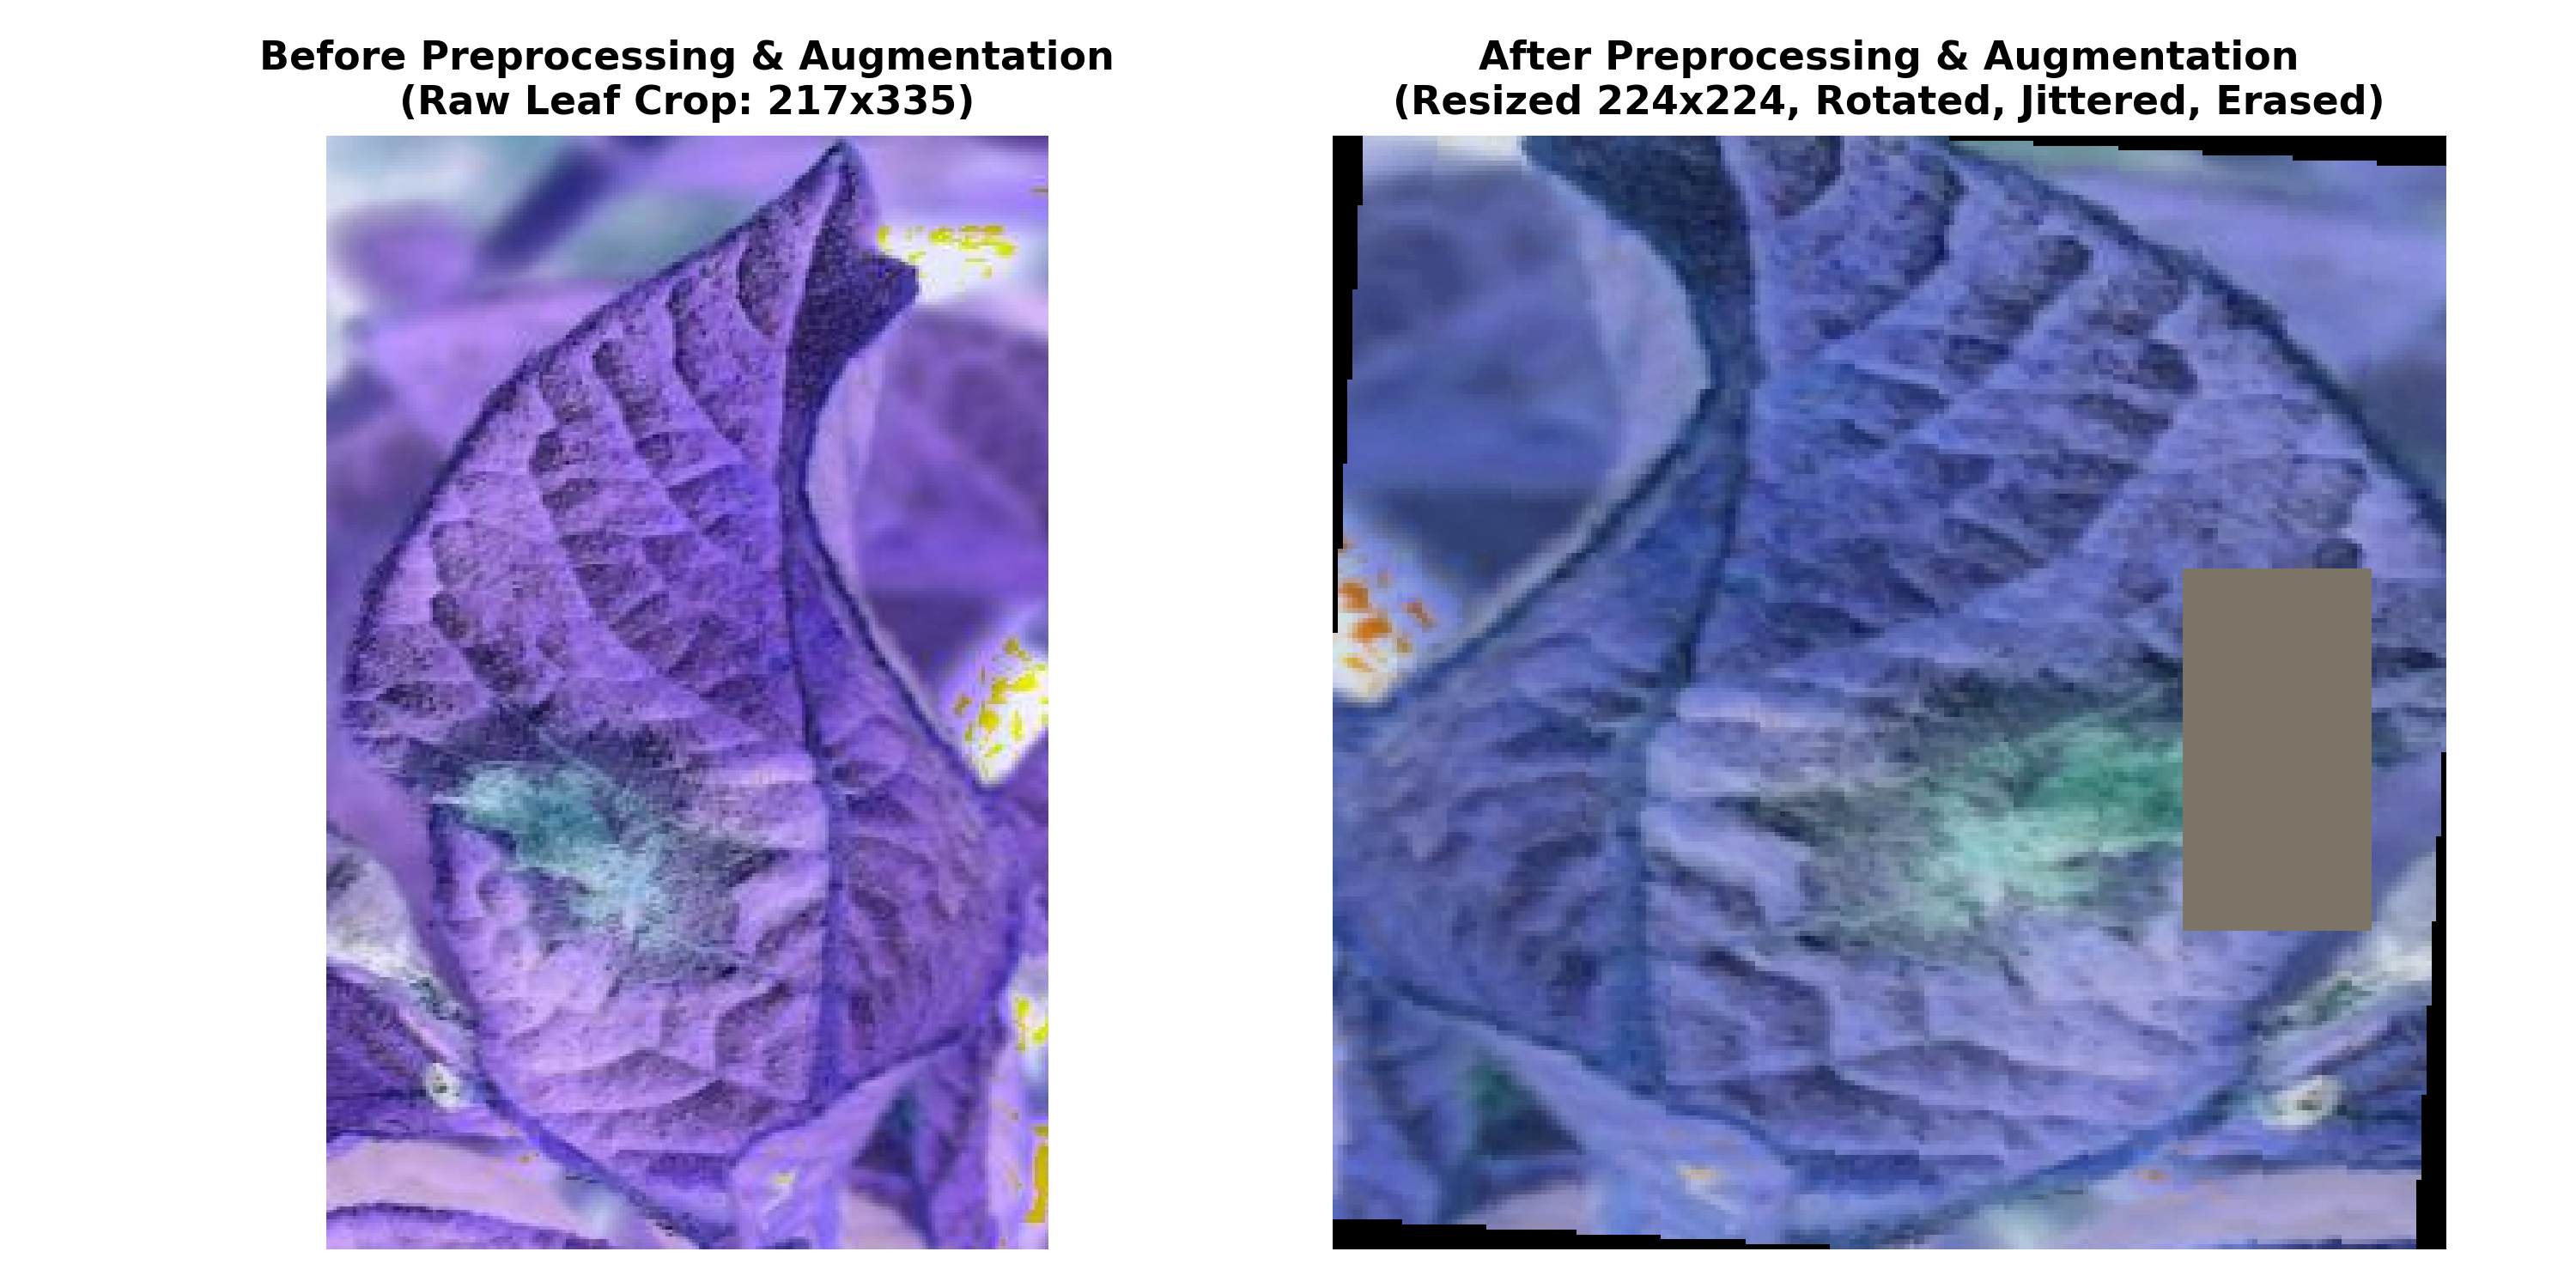
\includegraphics[width=0.85\linewidth]{figures/classification_preprocess_comparison.png}
    \caption{Classification: before and after preprocessing and augmentation.}
    \label{fig:cls_aug_example}
\end{figure}

\paragraph{Class Balancing with WeightedRandomSampler}

The PlantDoc dataset is significantly imbalanced.
Figure~\ref{fig:class_dist} shows the per-class instance counts before and after
applying \texttt{WeightedRandomSampler}: dominant classes (e.g.\ Blueberry leaf,
Tomato leaf) are down-weighted, while rare classes are up-weighted, producing a
roughly uniform sampling distribution across the 27 classes.

\begin{figure*}[t]
    \centering
    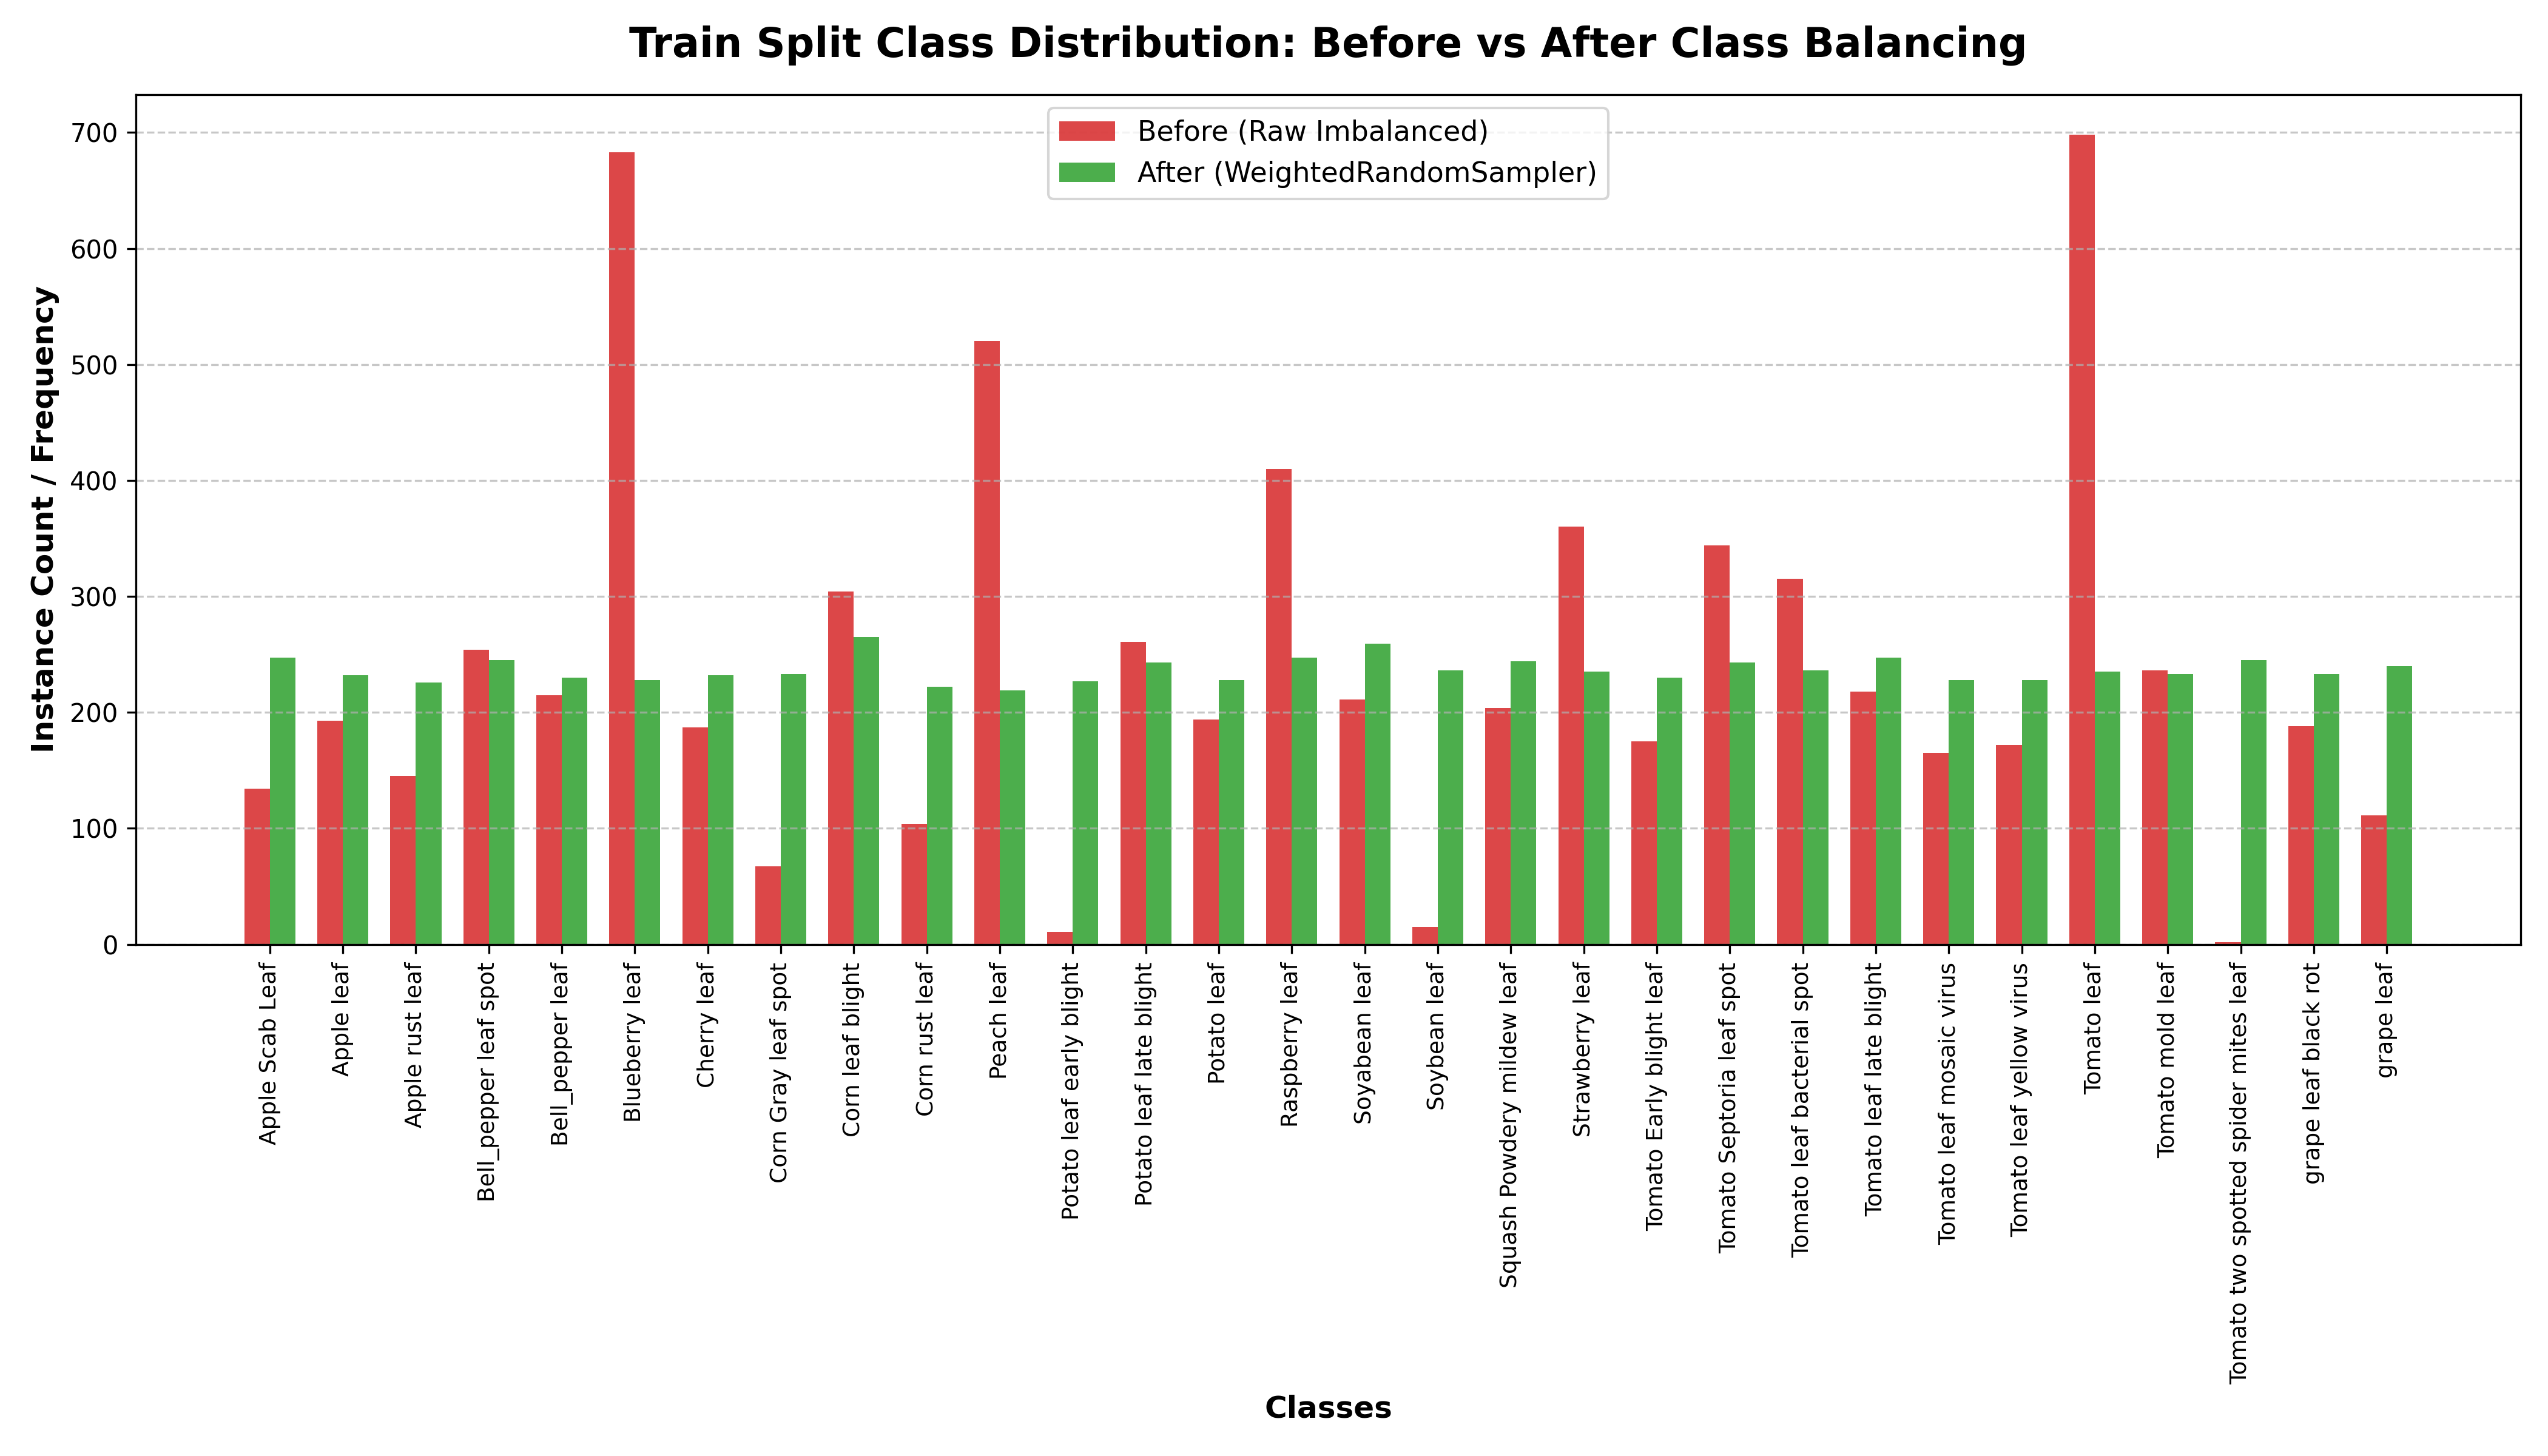
\includegraphics[width=0.85\linewidth]{figures/class_distribution_comparison.png}
    \caption{PlantDoc train-split class distribution before (red) and after (green) class balancing.}
    \label{fig:class_dist}
\end{figure*}

\subsubsection{Object Detection Pipeline}
\label{subsec:data_detection}

The preprocessing pipeline for the object detection task follows the YOLO
convention and comprises five stages (Figure~\ref{fig:det_pipeline}).

\begin{enumerate}
    \item \textbf{Input Data.}
          BGR images paired with normalised YOLO bounding box annotations.

    \item \textbf{Data Augmentation (training only).}
          Geometric transforms (rotation, flip, scale), colour and brightness
          adjustments, noise injection, and automatic bounding-box updates.

    \item \textbf{Preprocessing (training and inference).}
          \begin{itemize}
              \item Letterbox resize while preserving aspect ratio.
              \item Padding with grey value 114 to produce a square image.
              \item Colour-space conversion: BGR $\to$ RGB.
              \item Pixel normalisation to $[0.0,\, 1.0]$.
              \item Data-layout change: HWC $\to$ CHW.
          \end{itemize}

    \item \textbf{Output Tensor.}
          Image tensor of shape $(1,\, 3,\, \text{imgsz},\, \text{imgsz})$ with
          updated bounding boxes in YOLO format.

    \item \textbf{YOLO Model Input.}
          Ready for training or inference.
\end{enumerate}

\begin{figure*}[t]
    \centering
    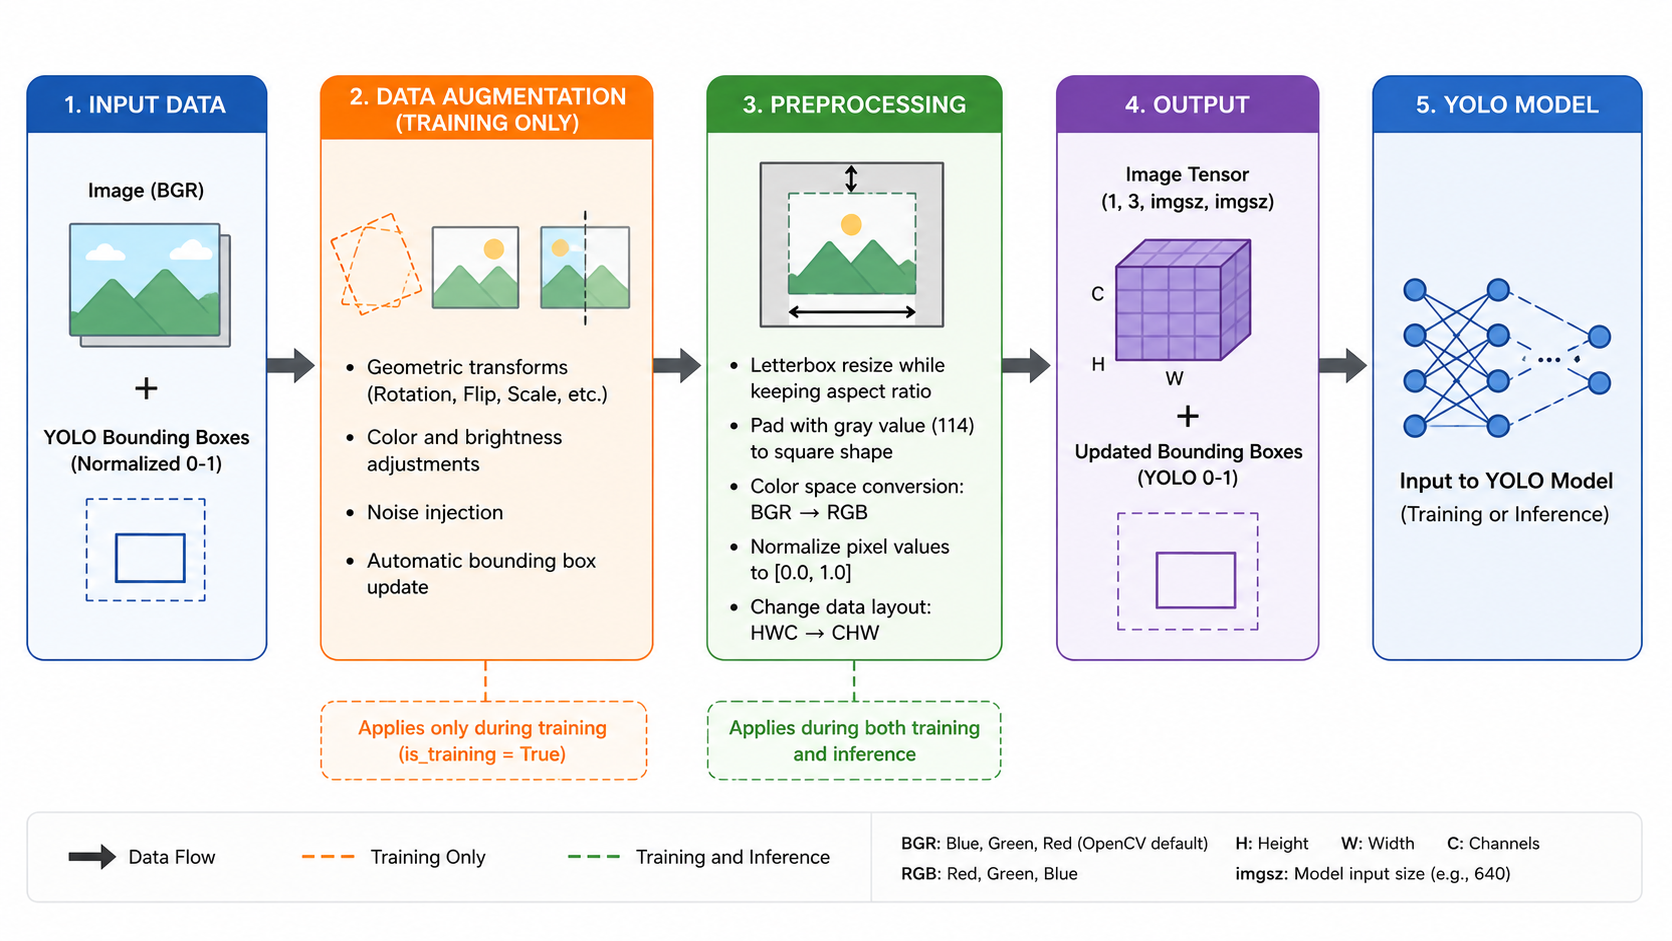
\includegraphics[width=0.85\linewidth]{figures/datapipeline_object.png}
    \caption{Data augmentation and preprocessing pipeline for the object detection task.}
    \label{fig:det_pipeline}
\end{figure*}

\paragraph{Visual Example}

Figure~\ref{fig:det_aug_example} shows a leaf image before (416$\times$416,
raw annotations, red bounding box) and after (resized to 640$\times$640, flipped,
colour-jittered, green bounding box) the detection pipeline.

\begin{figure}[!t]
    \centering
    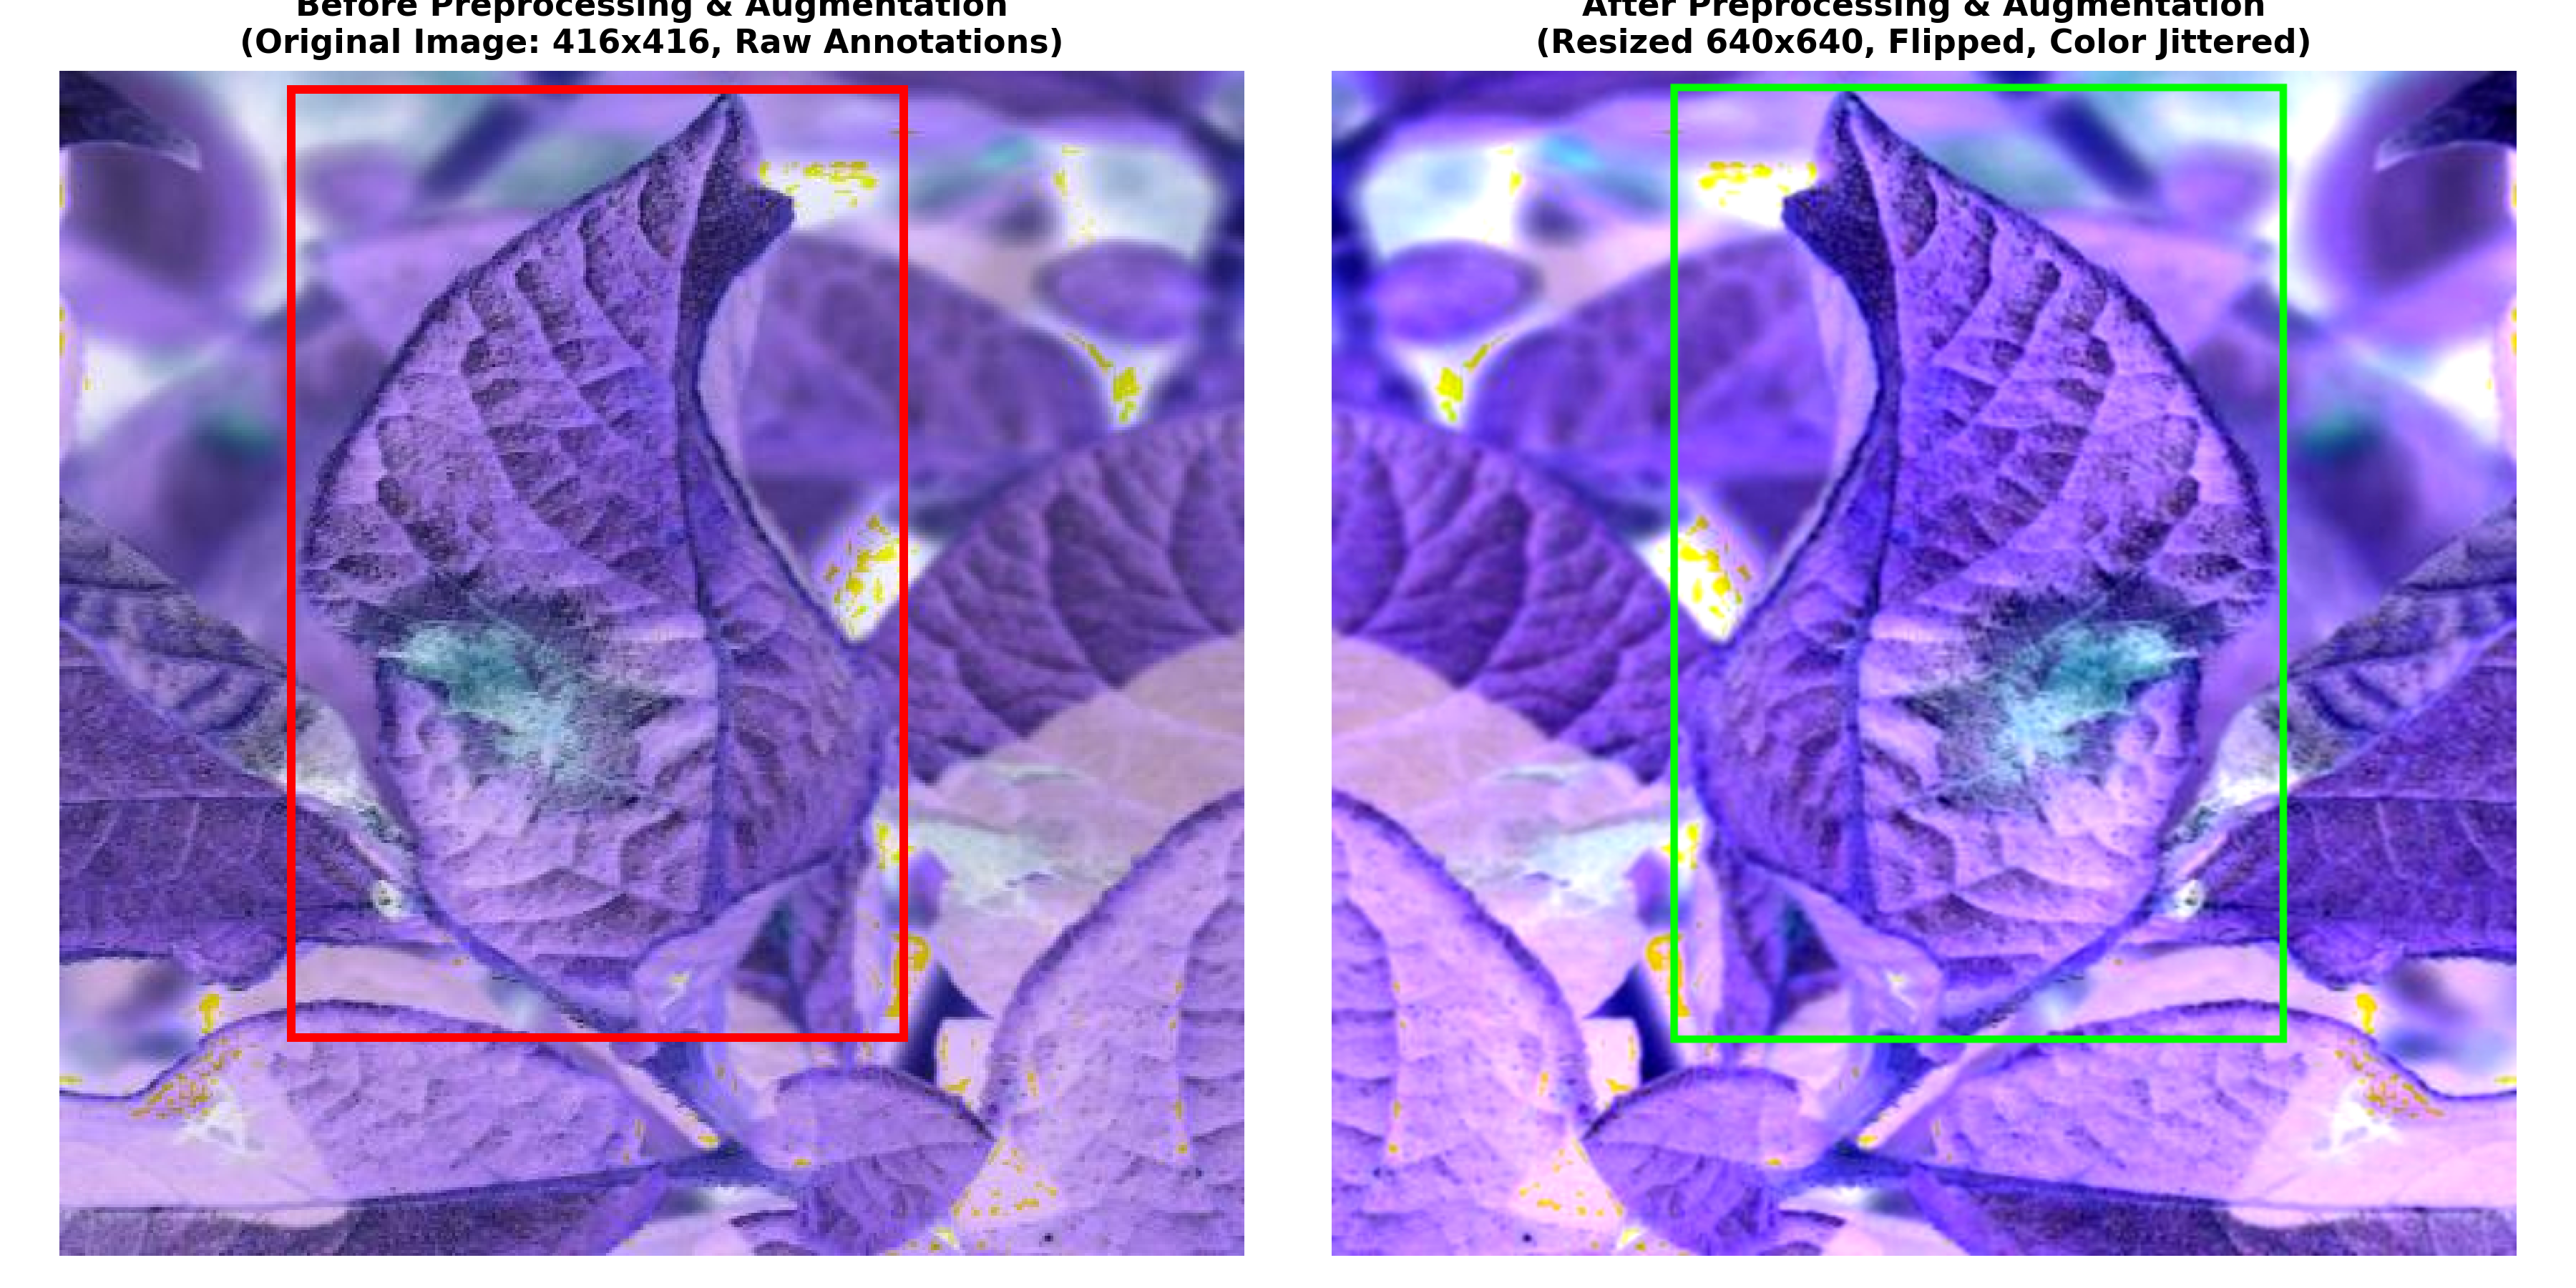
\includegraphics[width=0.85\linewidth]{figures/detection_preprocess_comparison.png}
    \caption{Object Detection: before and after preprocessing and augmentation.}
    \label{fig:det_aug_example}
\end{figure}

%% ============================================================
\subsection{Model Architectures}
\label{subsec:models}

This project implements and evaluates three published lightweight deep learning
architectures for plant leaf disease detection: (1) an Advanced Lightweight CNN
based on Depthwise Separable Convolutions with Squeeze-and-Excitation blocks
\cite{ashurov2025}, (2) V2PlantNet, an optimised MobileNet variant \cite{nnamdi2025},
and (3) YOLO-LeafNet, a YOLO-based object detection framework \cite{kaur2025}.

\subsubsection{Depthwise Separable Convolution}
\label{subsec:dwsconv}

Standard convolutions apply a single $D_k \times D_k$ filter simultaneously across
all $C_{in}$ input channels to produce each of the $C_{out}$ output feature maps.
The associated computational cost, denoted as $\text{Cost}_{\text{std}}$, is defined in (\ref{eq:cost_std}).
\begin{equation}
    \label{eq:cost_std}
    \text{Cost}_{\text{std}} = D_k \times D_k \times H \times W \times C_{in}
    \times C_{out}
\end{equation}

Depthwise Separable Convolution~\cite{ashurov2025} factorises this into two steps:

\begin{enumerate}
    \item \textbf{Depthwise Convolution.}
          A single $D_k \times D_k$ filter is applied to \emph{each} input channel
          independently (no cross-channel mixing), with the cost $\text{Cost}_{\text{dw}}$ given in (\ref{eq:cost_dw}).
          \begin{equation}
              \label{eq:cost_dw}
              \text{Cost}_{\text{dw}} = D_k \times D_k \times H \times W \times C_{in}
          \end{equation}

    \item \textbf{Pointwise Convolution} ($1{\times}1$).
          A $1\times1$ convolution combines the per-channel features into $C_{out}$
          output feature maps, with the cost $\text{Cost}_{\text{pw}}$ given in (\ref{eq:cost_pw}).
          \begin{equation}
              \label{eq:cost_pw}
              \text{Cost}_{\text{pw}} = H \times W \times C_{in} \times
              \frac{C_{out}}{G}
          \end{equation}
          where $G$ is the number of groups (set to 4 in the Advanced CNN).
\end{enumerate}

\subsubsection{Advanced Lightweight CNN}
\label{subsec:advanced_cnn}

The Advanced Lightweight CNN adapted from Ashurov et al.~\cite{ashurov2025} addresses edge deployment constraints by optimizing spatial feature extraction and attention calibration. Rather than utilizing standard 3D convolutions, the network is built on depthwise separable convolutions that factorize the convolution operation. To further minimize FLOPs and parameter footprint while ensuring channel interaction, grouped pointwise convolutions with a group size of $G=4$ are implemented.
To maximize feature discrimination under complex backgrounds, an enhanced Squeeze-and-Excitation (SE) block is integrated. The SE block squeezes spatial maps via Global Average Pooling and excites them using two fully-connected layers to compute channel-wise weights. Group Normalization (GN) is integrated within the block to replace Batch Normalization, ensuring stable training updates and channel recalibration under small-batch regimes. Finally, the network implements residual skip connections with depthwise convolutions along the shortcut paths to preserve gradient flow without inflating parameter overhead. The final feature representations pass through a fully connected layer and a dropout layer to output logits for multi-class classification.

The overall architecture is summarised in Figure~\ref{fig:advanced_cnn}.

\begin{figure}[!t]
    \centering
    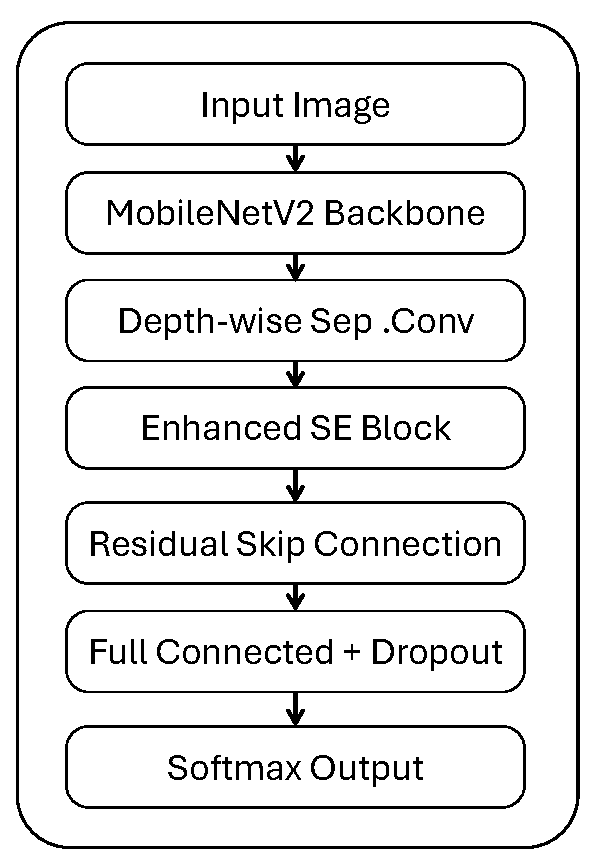
\includegraphics[width=0.6\linewidth]{figures/CNN_advance_cropped.pdf}
    \caption{Advanced Lightweight CNN Architecture~\cite{ashurov2025}.}
    \label{fig:advanced_cnn}
\end{figure}

\subsubsection{V2PlantNet}
\label{subsec:v2plantnet}

V2PlantNet~\cite{nnamdi2025} is an optimized, highly compact MobileNet-inspired classifier designed for real-time agricultural diagnostics on embedded systems. The network structure is designed to limit parameter count (0.38M parameters) and computational complexity (0.183 GFLOPs) through depthwise separable operations.
The model topology consists of:
\begin{enumerate}
    \item \textbf{Initial Stage}: A standard $3 \times 3$ convolutional layer with 32 filters, followed by Batch Normalization (BN) and ReLU activation to extract low-level features. A $3 \times 3$ Max Pooling layer with a stride of 2 then downsamples the feature maps.
    \item \textbf{Stage 1}: Comprises three Depthwise Separable Blocks with 64 output channels to capture detailed local visual structures.
    \item \textbf{Stage 2}: Comprises seven blocks with 128 output channels, utilizing a stride-2 pointwise convolution in the first block for spatial downsampling and receptive field expansion.
    \item \textbf{Stage 3}: Comprises three blocks with 256 output channels, capturing high-level abstract semantic features.
    \item \textbf{Final Classification Stage}: Utilizes a Global Average Pooling (GAP) layer to reduce the 3D feature maps to a 256-dimensional vector, mitigating overfitting. This vector is passed to a fully connected layer (256 units), regularized via a Dropout layer (rate 0.45), and mapped to the final classification layer with Softmax activation.
\end{enumerate}

The V2PlantNet architecture is illustrated in Figure~\ref{fig:v2plantnet}.

\begin{figure*}[t]
    \centering
    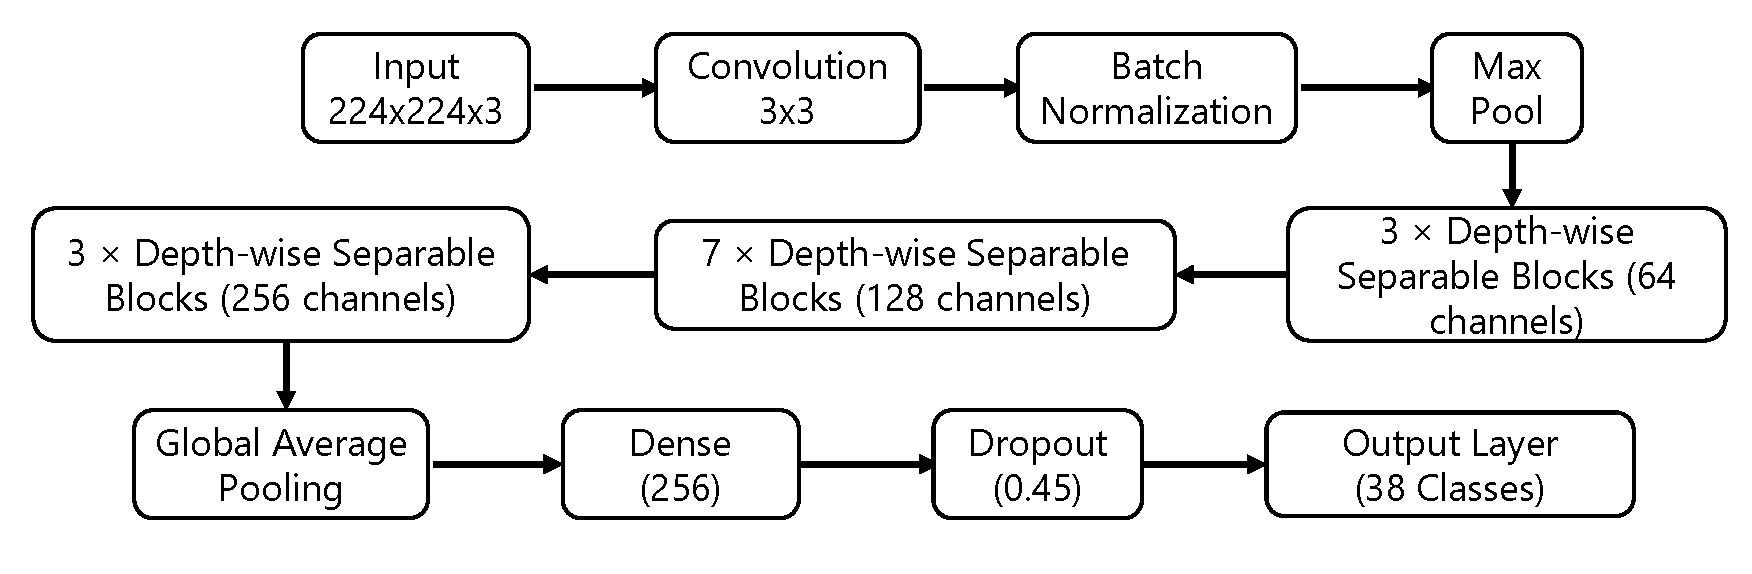
\includegraphics[width=0.6\linewidth]{figures/PlantNet_cropped.pdf}
    \caption{V2PlantNet Architecture~\cite{nnamdi2025}.}
    \label{fig:v2plantnet}
\end{figure*}

\subsubsection{YOLO-LeafNet}
\label{subsec:yolo_leafnet}

YOLO-LeafNet~\cite{kaur2025} is a robust deep learning framework designed for real-time multispecies plant disease detection, allowing simultaneous localization and multi-class identification.
The network architecture is organized into three main modules:
\begin{itemize}
    \item \textbf{Backbone}: Based on CSPDarknet53 from YOLOv8, it utilizes convolutional layers and C2f (Cross-Stage Partial Bottleneck with two convolutions) modules for hierarchical feature extraction. To prevent overfitting under real-world noise, YOLO-LeafNet integrates Batch Normalization and Dropout layers directly into the backbone. A Spatial Pyramid Pooling Fast (SPPF) module is positioned at the end of the backbone to aggregate context across multiple receptive fields.
    \item \textbf{Neck}: Adopts a Path Aggregation Network (PANet) or Feature Pyramid Network (FPN) structure. It fuses high-level semantic features and low-level spatial features through top-down and bottom-up pathways using upsampling, downsampling, and concatenation, enabling multi-scale feature fusion.
    \item \textbf{Head}: Uses an anchor-free design that predicts bounding boxes and class probabilities directly via three detection branches operating at different scales (e.g., resolutions of $72 \times 72$, $36 \times 36$, and $18 \times 18$). This multi-scale detection allows YOLO-LeafNet to identify very small early-stage lesions as well as large infected zones.
\end{itemize}

The YOLO-LeafNet architecture based on YOLOv8 is shown in Figure~\ref{fig:yolo_leafnet_v8}.

\begin{figure*}[t]
    \centering
    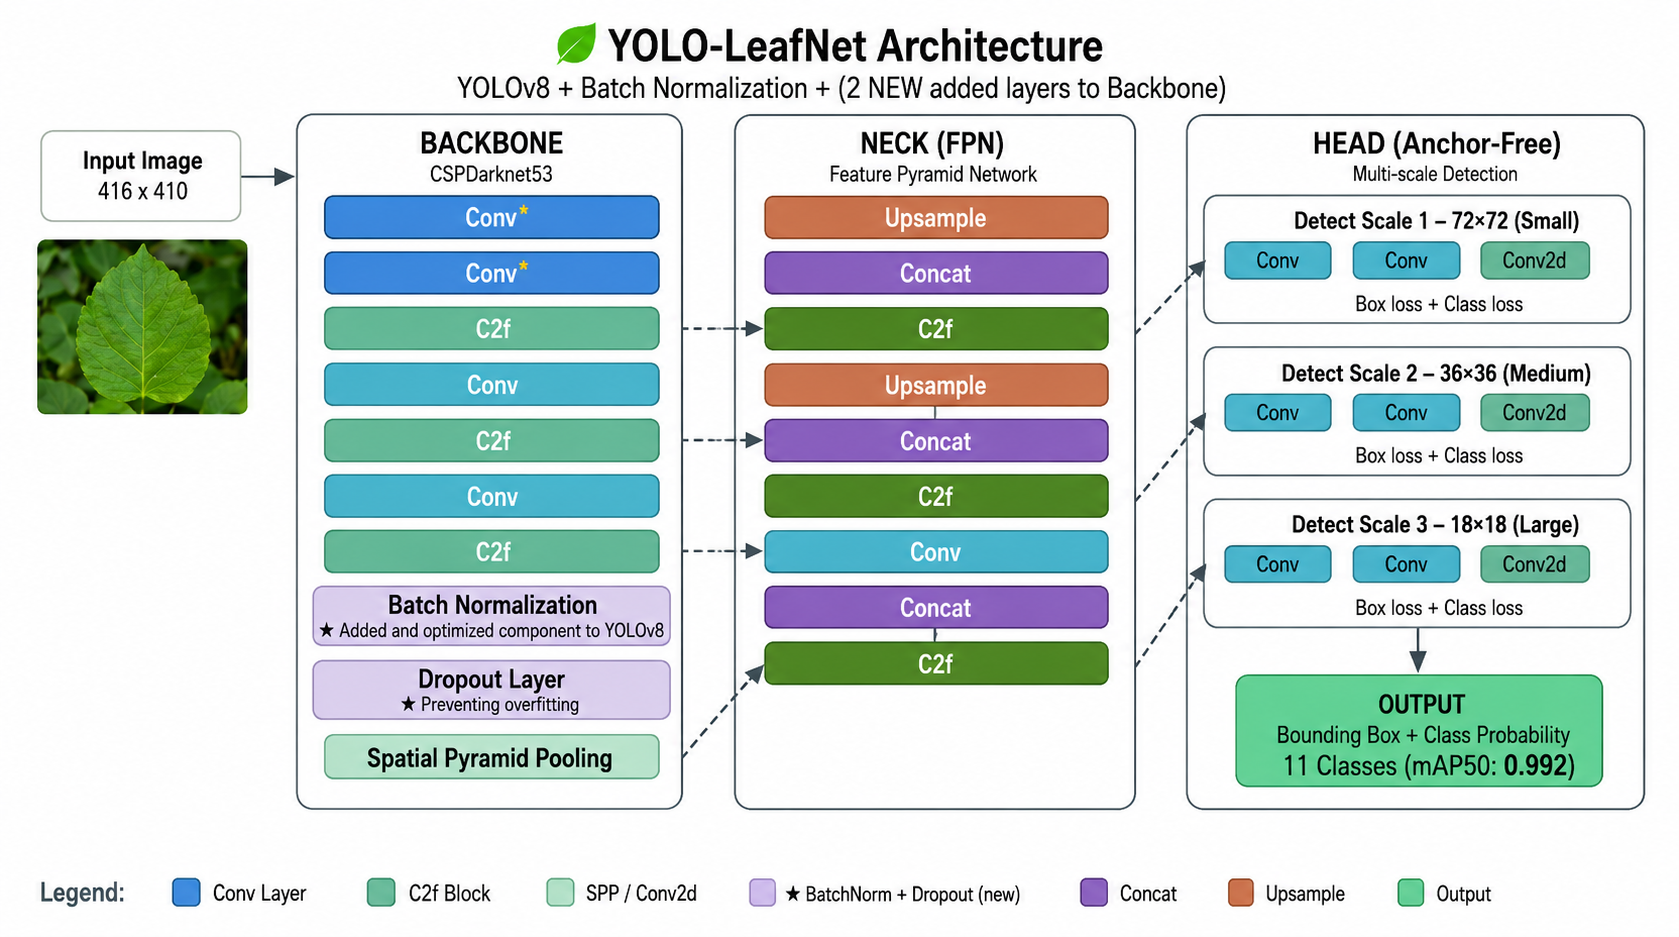
\includegraphics[width=0.85\linewidth]{figures/Yololeafnet.png}
    \caption{YOLO-LeafNet architecture based on YOLOv8~\cite{kaur2025}.}
    \label{fig:yolo_leafnet_v8}
\end{figure*}

Published performance on the original test set~\cite{kaur2025}:
\begin{itemize}
    \item YOLOv5: Precision 0.861, Recall 0.868, mAP@50 0.944.
    \item YOLOv8: Precision 0.977, Recall 0.975, mAP@50 0.984.
    \item YOLO-LeafNet: \textbf{Precision 0.985, Recall 0.980,
          mAP@50 0.990}.
\end{itemize}

\paragraph{Architecture with YOLOv12S Backbone}

The YOLOv12S backbone version restructures the neck into explicit
\emph{upsampling} (FPN top-down) and \emph{downsampling} (PAN bottom-up) paths,
providing richer multi-scale feature fusion, as illustrated in Figure~\ref{fig:yolo_leafnet_v12}.

\begin{figure*}[!t]
    \centering
    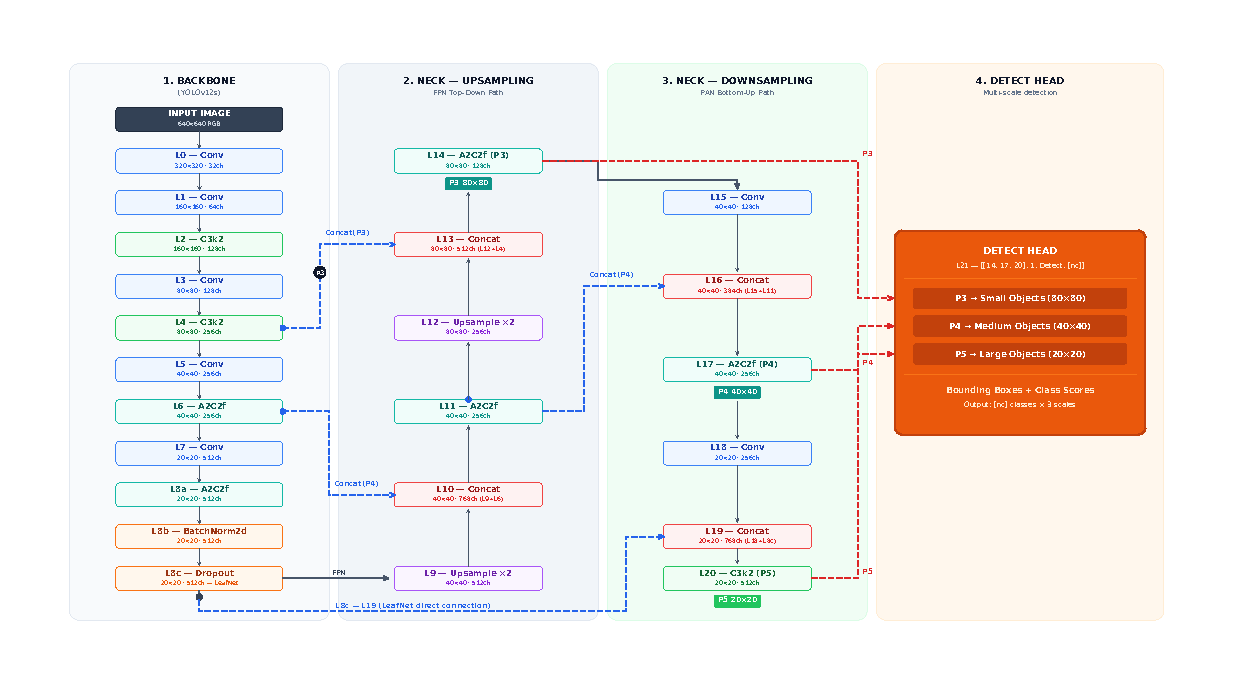
\includegraphics[width=0.85\linewidth]{figures/YOLOv12s_LeafNet_Architecture_cropped.pdf}
    \caption{YOLO-LeafNet with YOLOv12S Backbone~\cite{kaur2025}.}
    \label{fig:yolo_leafnet_v12}
\end{figure*}

%% ============================================================
\section{Results and Discussion}
\label{sec:results}

\subsection{Evaluation Metrics}
\label{subsec:metrics}

To rigorously evaluate the models on classification and detection tasks, we employ standard performance and operational metrics that align with our experimental results.

\subsubsection{Classification Performance Metrics}

\paragraph{Accuracy}
Accuracy represents the overall fraction of correctly classified leaf samples across all classes, as calculated in (\ref{eq:accuracy}).
\begin{equation}
    \label{eq:accuracy}
    \text{Accuracy} = \frac{1}{N}\sum_{i=1}^{N} \mathbb{I}\!\left(\hat{y}_i = y_i\right)
\end{equation}
where $\hat{y}_i$ is the predicted class, $y_i$ is the ground-truth label, and $\mathbb{I}$ is the indicator function.

\paragraph{Precision and Recall}
Precision measures the reliability of positive predictions (minimizing false alarms), while Recall measures the sensitivity to detect all diseased leaf instances, as shown in (\ref{eq:precision_recall}).
\begin{equation}
    \label{eq:precision_recall}
    \text{Precision} = \frac{TP}{TP + FP}, \qquad \text{Recall} = \frac{TP}{TP + FN}
\end{equation}
where $TP$, $FP$, and $FN$ represent true positives, false positives, and false negatives.

\paragraph{F1-Score}
The F1-score is the harmonic mean of Precision and Recall, balancing the two metrics as defined in (\ref{eq:f1}).
\begin{equation}
    \label{eq:f1}
    F_1 = 2 \times \frac{\text{Precision} \times \text{Recall}}{\text{Precision} + \text{Recall}}
\end{equation}

\subsubsection{Detection and Localisation Metrics}

\paragraph{Intersection over Union (IoU)}
IoU measures the spatial overlap between the predicted bounding box $B_{\text{pred}}$ and the ground-truth bounding box $B_{\text{gt}}$ according to (\ref{eq:iou}).
\begin{equation}
    \label{eq:iou}
    \text{IoU} = \frac{\text{Area}(B_{\text{pred}} \cap B_{\text{gt}})}{\text{Area}(B_{\text{pred}} \cup B_{\text{gt}})}
\end{equation}

\paragraph{Mean Average Precision (mAP)}
Object detection performance is measured using Mean Average Precision. The Average Precision (AP) for class $k$ is calculated as the area under the precision-recall curve $p(r)$, as defined in (\ref{eq:ap}).
\begin{equation}
    \label{eq:ap}
    \text{AP}_k = \int_0^1 p(r)\, dr
\end{equation}
The mAP is computed by averaging $\text{AP}_k$ across all $K$ classes in (\ref{eq:map}).
\begin{equation}
    \label{eq:map}
    \text{mAP} = \frac{1}{K}\sum_{k=1}^{K} \text{AP}_k
\end{equation}
We report two specific metrics: \textbf{mAP@50} (where a predicted box is counted as positive if its $\text{IoU} \ge 0.50$) and \textbf{mAP@50-95} (the average mAP calculated over ten IoU thresholds from 0.50 to 0.95 with step size 0.05).

\subsubsection{Operational Metrics}

For real-world deployment on mobile or edge platforms, we track efficiency and complexity:

\paragraph{Inference Latency}
Inference latency measures the time (in milliseconds) required to process a single image, as expressed in (\ref{eq:latency}).
\begin{equation}
    \label{eq:latency}
    \text{Latency} = T_{\mathrm{end}} - T_{\mathrm{start}}
\end{equation}

\paragraph{Model Complexity}
Model size is quantified by the total number of trainable parameters according to (\ref{eq:params}).
\begin{equation}
    \label{eq:params}
    \text{Total Parameters} = \sum_{l=1}^{L} \left( w_l + b_l \right)
\end{equation}
where $w_l$ and $b_l$ are the number of weights and biases in layer $l$, and $L$ is the total number of layers.

%% ============================================================
\subsection{Experimental Settings}
\label{subsec:settings}

\subsubsection{Development Environment}

\begin{itemize}
    \item \textbf{Deep Learning Framework:} PyTorch 2.8.0
    \item \textbf{Object Detection Library:} Ultralytics (YOLO) 8.4.56
    \item \textbf{Hardware:} Kaggle GPU T4 $\times$ 2 (Dual T4)
\end{itemize}

\subsubsection{Model and Task Configurations}

\begin{itemize}
    \item \textbf{Input Resolution:}
    \begin{itemize}
        \item Classification: $224 \times 224$ pixels
        \item Object Detection: $640 \times 640$ pixels
    \end{itemize}
    \item \textbf{Regularisation:} Dropout $= 0.3$ (applied to the LeafNet
          architecture)
\end{itemize}

\subsubsection{Training Hyperparameters}

The training hyperparameters used across all experiments are detailed in Table~\ref{tab:hyperparams}.

\begin{table}[!t]
    \centering
    \caption{Training hyperparameters used across all experiments.}
    \label{tab:hyperparams}
    \begin{tabular}{ll}
        \toprule
        \textbf{Hyperparameter}   & \textbf{Value} \\
        \midrule
        Optimiser                 & AdamW \\
        Base Learning Rate        & 0.001 \\
        LR Scheduler              & Cosine Annealing \\
        Batch Size (Classification)  & 32 \\
        Batch Size (Object Detection) & 16 \\
        Weight Decay              & 0.0005 \\
        Early Stopping Patience   & 15 epochs \\
        \midrule
        Training Epochs — PlantVillage & 10 \\
        Training Epochs — PlantDoc     & 50 \\
        \bottomrule
    \end{tabular}
\end{table}

%% ============================================================
\subsection{Performance Evaluation}
\label{subsec:results}

\subsubsection{Results on PlantVillage}
\label{subsec:results_plantvillage}

\paragraph{Classification}

The classification results on the PlantVillage dataset are presented in Table~\ref{tab:cls_plantvillage}. The evaluated architectures show exceptional performance on this dataset. Specifically, the Advanced Lightweight CNN achieves the highest diagnostic capability, registering a classification accuracy of 99.05\%, along with a precision of 99.06\% and a recall of 99.03\%. The ultra-lightweight V2PlantNet model shows slightly lower but highly competitive performance, yielding 98.31\% accuracy. The high accuracy across both models is primarily attributed to the high-contrast, uniform backgrounds of the laboratory-captured PlantVillage images, which simplify classification by minimizing confounding background clutter.

\begin{table*}[t]
    \centering
    \caption{Classification results on PlantVillage dataset.}
    \label{tab:cls_plantvillage}
    \setlength{\tabcolsep}{5pt}
    \begin{tabular}{lccccc}
        \toprule
        \textbf{Architecture} & \textbf{Accuracy} & \textbf{Precision}
                              & \textbf{Recall} & \textbf{F1}
                              & \textbf{Inference (ms)} \\
        \midrule
        CNN Advance
            & \textcolor{bestred}{\textbf{99.05\%}}
            & \textcolor{bestred}{\textbf{99.06\%}}
            & \textcolor{bestred}{\textbf{99.03\%}}
            & \textcolor{bestred}{\textbf{99.03\%}}
            & 0.17 \\
        V2PlantNet
            & 98.31\% & 98.33\% & 98.38\% & 98.27\% & \textcolor{bestred}{\textbf{0.08}} \\
        \bottomrule
    \end{tabular}\\[4pt]
    {\small \textcolor{bestred}{Red}: best results.}
\end{table*}

\paragraph{Object Detection}

The object detection results on the PlantVillage dataset are summarized in Table~\ref{tab:det_plantvillage}. Across all models, detection mean Average Precision (mAP@50) remains exceptionally high, exceeding 99.4\%. Standard YOLOv12s leads the benchmark with a mAP@50 of 99.49\% and an F1-score of 99.75\%, utilizing 9.25 million parameters. The YOLO-LeafNet modifications based on YOLOv8 and YOLOv12s exhibit identical mAP@50 scores of 99.45\%. The results demonstrate that lightweight object detection architectures are highly capable of localizing disease symptoms when the image features are distinct and captured under controlled laboratory settings.

\begin{table*}[t]
    \centering
    \caption{Object detection results on PlantVillage dataset.}
    \label{tab:det_plantvillage}
    \setlength{\tabcolsep}{4pt}
    \begin{tabular}{lcccccc}
        \toprule
        \textbf{Architecture} & \textbf{mAP@50} & \textbf{Prec.}
                              & \textbf{Recall} & \textbf{F1}
                              & \textbf{mAP@50-95} & \textbf{Params} \\
        \midrule
        YOLOv8s-LeafNet
            & \textcolor{bestred}{\textbf{99.45\%}} & 99.43\% & 99.06\% & 99.24\%
            & 98.94\% & 11.14 M \\
        YOLOv12s-LeafNet
            & \textcolor{bestred}{\textbf{99.45\%}} & 99.39\% & \textcolor{bestred}{\textbf{99.48\%}} & 99.43\%
            & 99.02\% & 9.25 M \\
        YOLOv12s
            & \textcolor{bestred}{\textbf{99.49\%}} & \textcolor{bestred}{\textbf{99.77\%}} & \textcolor{bestred}{\textbf{99.72\%}}
            & \textcolor{bestred}{\textbf{99.75\%}}
            & \textcolor{bestred}{\textbf{99.16\%}} & 9.25 M \\
        YOLOv5s
            & 99.47\% & 99.48\% & 99.53\% & 99.50\% & 98.89\% & 9.1 M \\
        \bottomrule
    \end{tabular}\\[4pt]
    {\small \textcolor{bestred}{Red}: best results.}
\end{table*}

\paragraph{Confusion Matrices}

The confusion matrices for the evaluated models on the PlantVillage dataset are compared in Figure~\ref{fig:cm_plantvillage}. The visual representations reveal a highly diagonal structure across all model configurations, indicating negligible misclassification rates. For the Advanced CNN, misclassification is restricted to subtle confusions between highly similar diseases within the same plant family, such as distinguishing between early stages of Tomato Early Blight and Tomato Late Blight. In V2PlantNet, a minor rate of off-diagonal confusion is observed between different healthy categories (e.g., healthy Apple leaf versus healthy Peach leaf) when leaves share similar shapes. However, the strong diagonal clustering confirms that isolated backgrounds and uniform illumination enable the lightweight models to establish sharp decision boundaries with minimal inter-class overlap.

\begin{figure*}[!t]
    \centering
    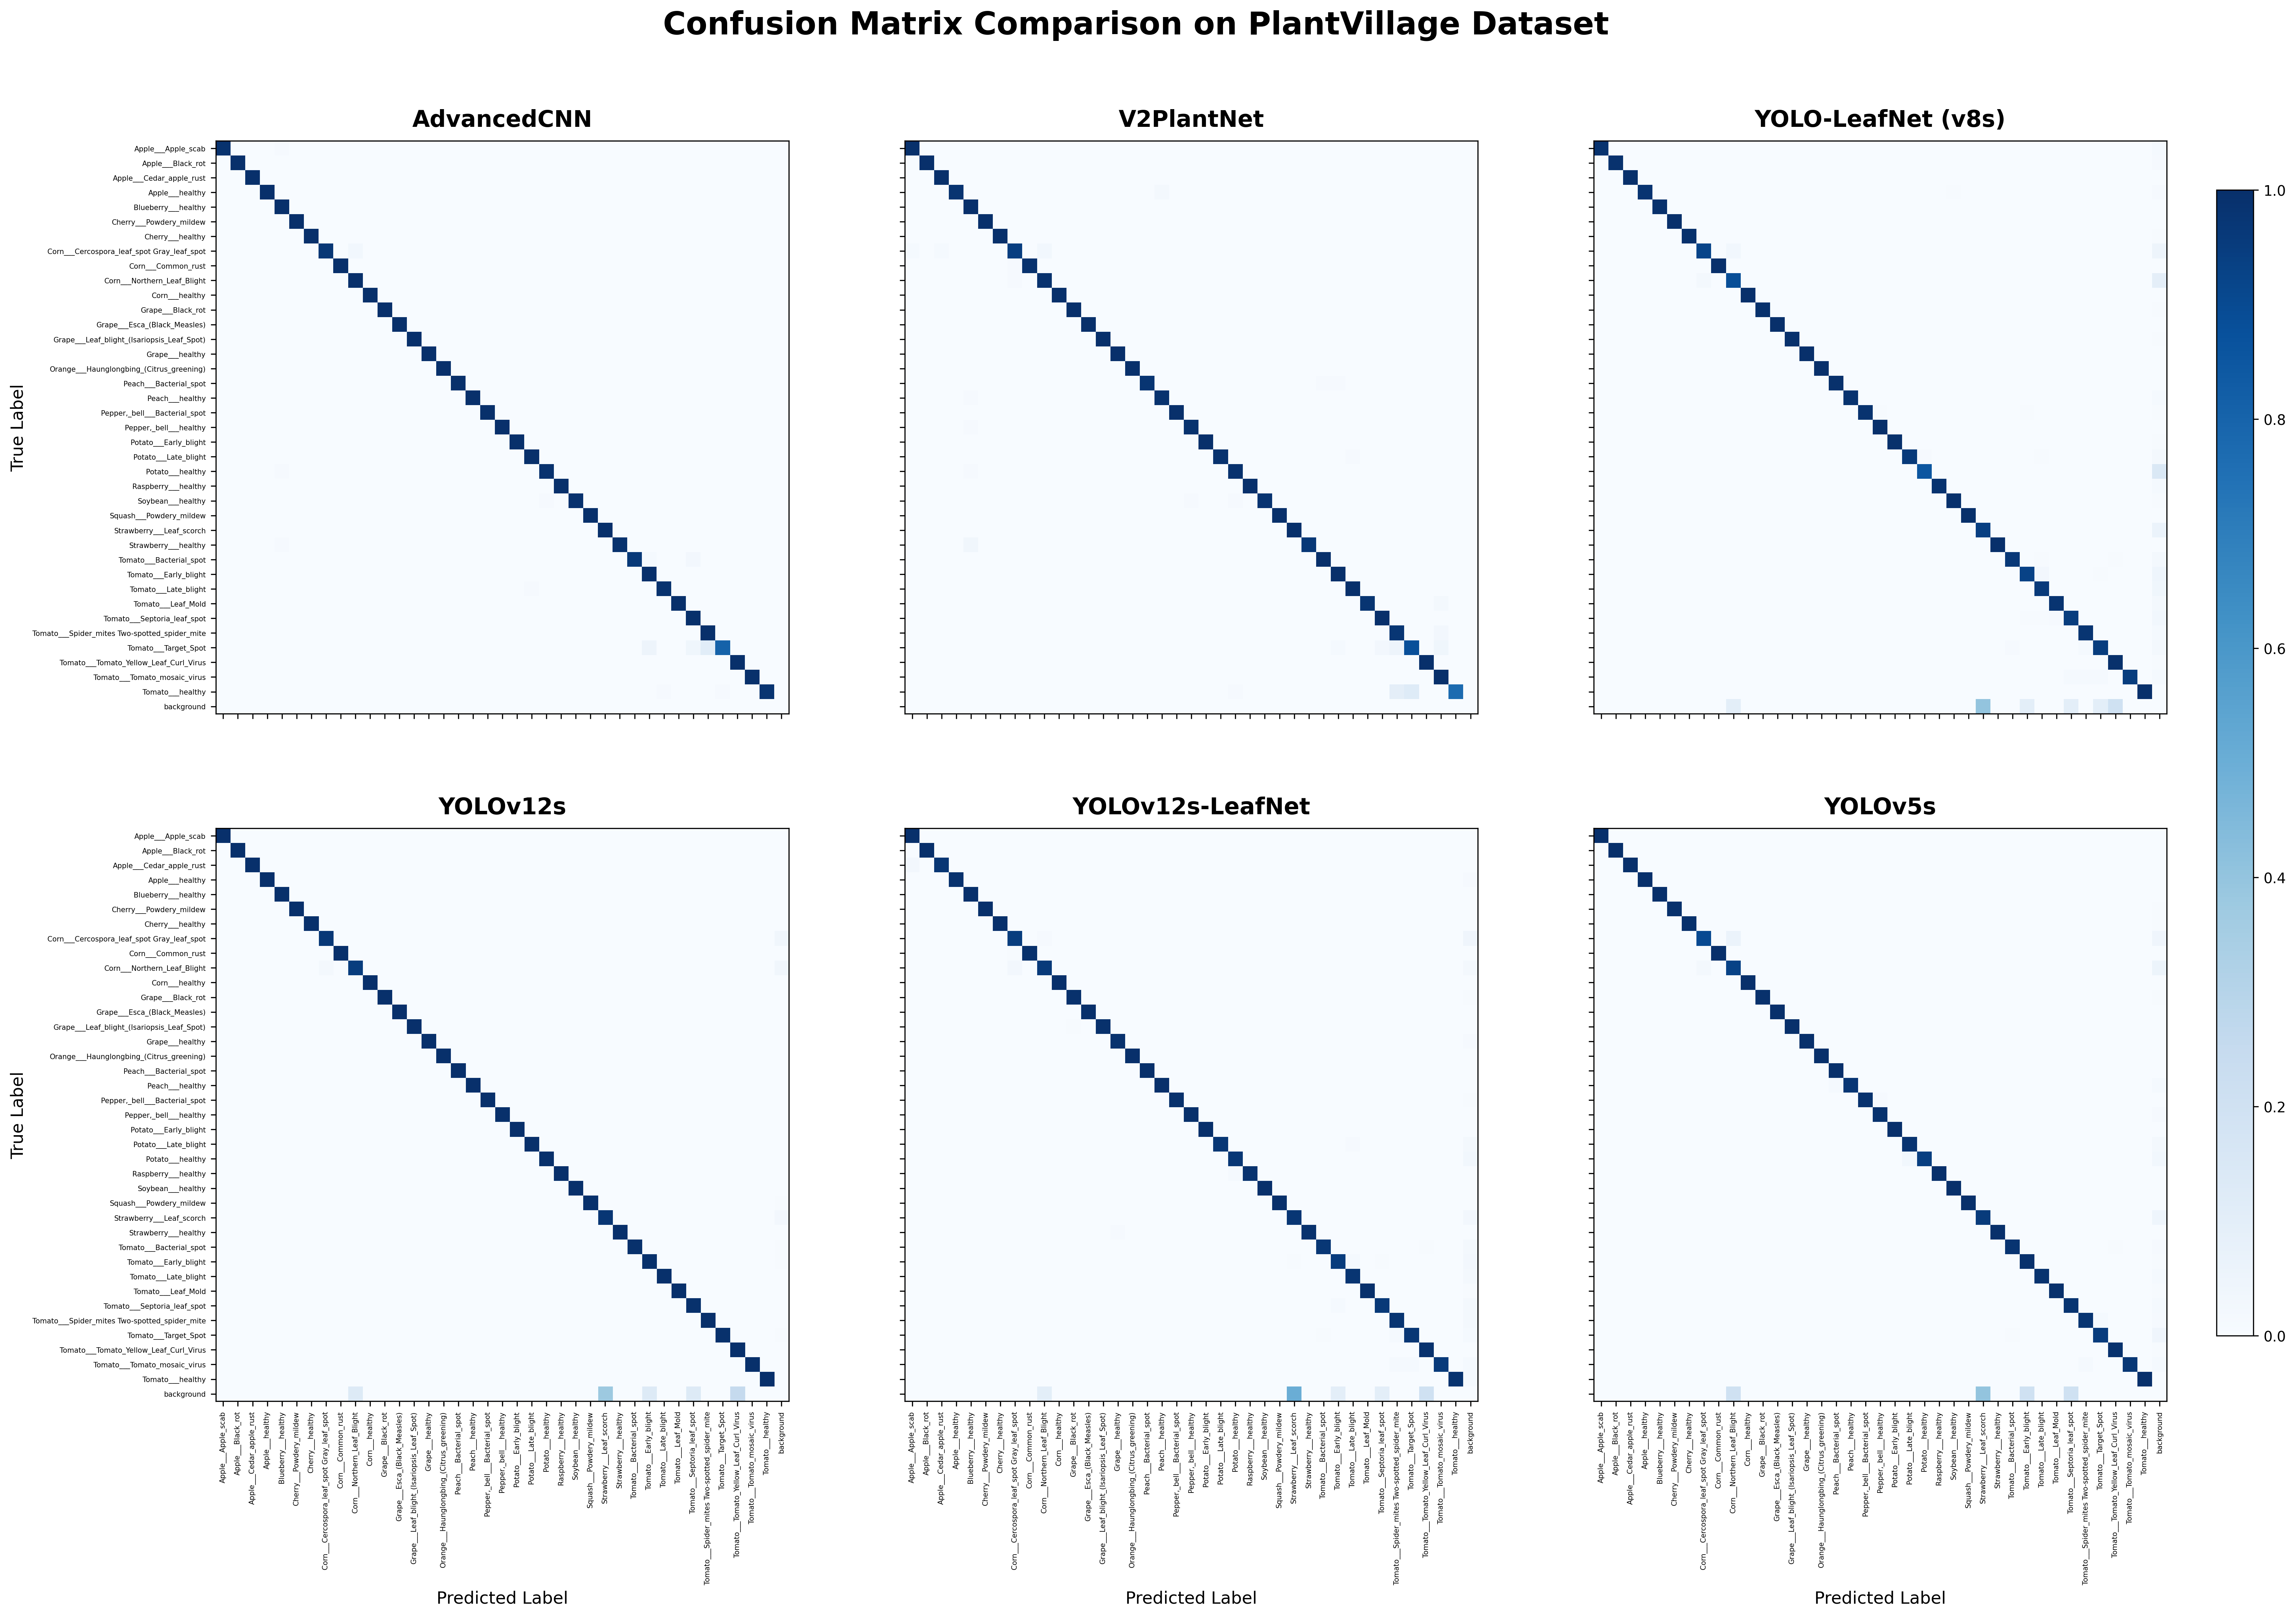
\includegraphics[width=0.8\linewidth]{figures/combined_confusion_matrix_plantvillage.png}
    \caption{Confusion matrix comparison on PlantVillage.}
    \label{fig:cm_plantvillage}
\end{figure*}

\subsubsection{Results on PlantDoc}
\label{subsec:results_plantdoc}

\paragraph{Classification}

The classification results on the PlantDoc dataset are shown in Table~\ref{tab:cls_plantdoc}. Unlike the controlled PlantVillage dataset, the unstructured nature of the PlantDoc images introduces severe noise. Under these conditions, classification performance degrades significantly. The Advanced CNN records a classification accuracy of only 53.96\%, whereas the ultra-lightweight V2PlantNet drops further to 46.26\%. Despite its lower accuracy, V2PlantNet maintains a significant latency advantage (8.69 ms vs. 18.30 ms), rendering it highly attractive for environments with stringent processing constraints.

\begin{table*}[t]
    \centering
    \caption{Classification results on PlantDoc dataset.}
    \label{tab:cls_plantdoc}
    \setlength{\tabcolsep}{5pt}
    \begin{tabular}{lccccc}
        \toprule
        \textbf{Architecture} & \textbf{Accuracy} & \textbf{Precision}
                              & \textbf{Recall} & \textbf{F1}
                              & \textbf{Inference (ms)} \\
        \midrule
        CNN Advance
            & \textcolor{bestred}{\textbf{53.96\%}}
            & \textcolor{bestred}{\textbf{52.50\%}}
            & \textcolor{bestred}{\textbf{55.79\%}}
            & \textcolor{bestred}{\textbf{52.14\%}}
            & 18.30 \\
        V2PlantNet
            & 46.26\% & 41.39\% & 42.90\% & 40.11\% & \textcolor{bestred}{\textbf{8.69}} \\
        \bottomrule
    \end{tabular}\\[4pt]
    {\small \textcolor{bestred}{Red}: best results.}
\end{table*}

\paragraph{Object Detection}

The object detection results on the PlantDoc dataset are summarized in Table~\ref{tab:det_plantdoc}. Standard YOLOv12s achieves the highest localization capability with a mAP@50 of 63.65\% and a recall of 67.51\%, using 9.2M parameters. The YOLOv8s-LeafNet model records a mAP@50 of 56.51\% while yielding the highest precision of 57.49\%. In contrast, YOLOv12s-LeafNet yields a lower mAP@50 of 44.75\%, indicating that the specific architectural modifications of LeafNet were less robust to the severe background noise, occlusions, and multi-scale variations present in the raw, field-collected images compared to the baseline models.

\begin{table*}[t]
    \centering
    \caption{Object detection results on PlantDoc dataset.}
    \label{tab:det_plantdoc}
    \setlength{\tabcolsep}{4pt}
    \begin{tabular}{lcccccc}
        \toprule
        \textbf{Architecture} & \textbf{mAP@50} & \textbf{Prec.}
                              & \textbf{Recall} & \textbf{F1}
                              & \textbf{mAP@50-95} & \textbf{Params} \\
        \midrule
        YOLOv8s-LeafNet
            & 56.51\% & \textcolor{bestred}{\textbf{57.49\%}} & 52.28\% & 54.76\%
            & 43.13\% & 11.14 M \\
        YOLOv12s-LeafNet
            & 44.75\% & 32.70\% & 50.90\% & 39.82\% & 34.56\% & 9.24 M \\
        YOLOv12s
            & \textcolor{bestred}{\textbf{63.65\%}} & 52.52\%
            & \textcolor{bestred}{\textbf{67.51\%}}
            & \textcolor{bestred}{\textbf{59.08\%}}
            & \textcolor{bestred}{\textbf{49.94\%}} & 9.2 M \\
        YOLOv5s
            & 63.13\% & 57.59\% & 63.47\% & 60.39\% & 48.38\% & 9.1 M \\
        \bottomrule
    \end{tabular}\\[4pt]
    {\small \textcolor{bestred}{Red}: best results.}
\end{table*}

\paragraph{Confusion Matrices}

The confusion matrices comparing model performance on the PlantDoc dataset are shown in Figure~\ref{fig:cm_plantdoc}. Under real-world noise, the confusion matrices show a high level of off-diagonal scattering, demonstrating substantial classification ambiguity. A critical pattern of misclassification occurs between early-stage fungal diseases (e.g., Apple Rust, Corn Gray Leaf Spot) and healthy leaves, as small lesions are often obscured by background foliage or variable shadows. Additionally, significant inter-species confusion is observed, where structurally similar leaves of different crops (such as Tomato and Potato leaves) are misclassified. This is exacerbated by the severe class imbalance of the PlantDoc set, which biases models toward predicting dominant classes (such as Blueberry and Tomato) and results in elevated off-diagonal rates in these specific columns.

\begin{figure*}[!t]
    \centering
    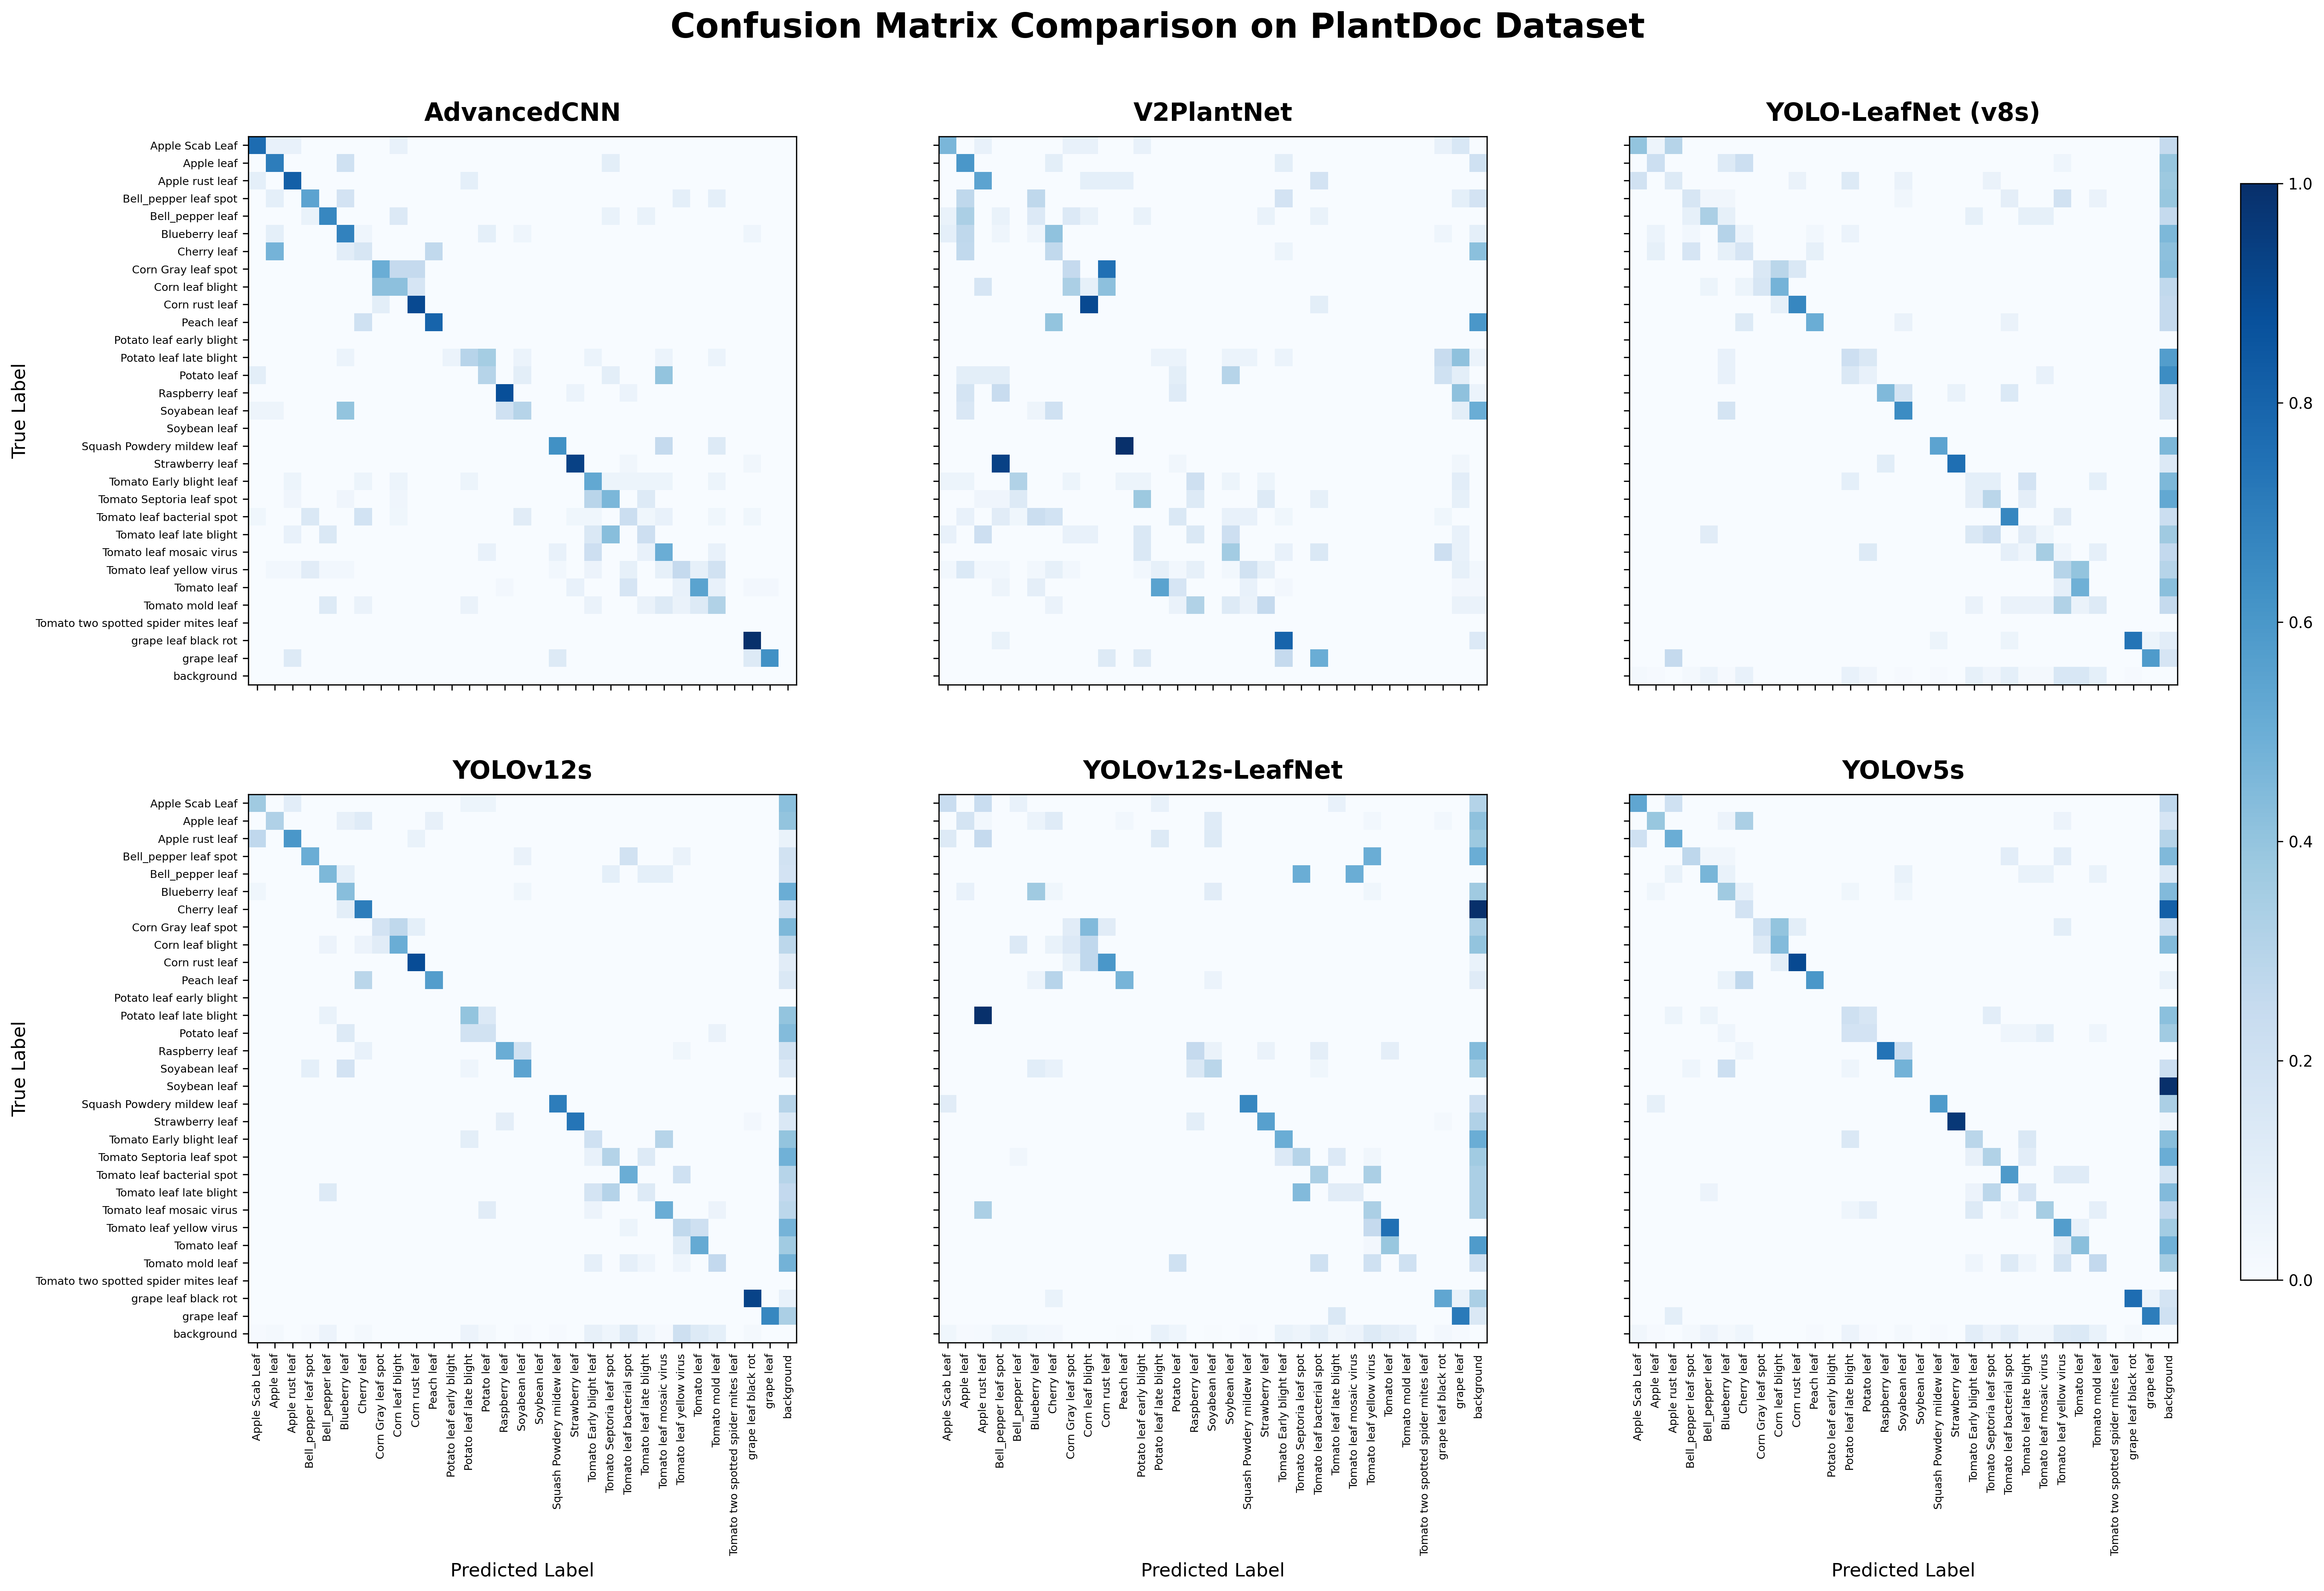
\includegraphics[width=0.8\linewidth]{figures/combined_confusion_matrix_plantdoc.png}
    \caption{Confusion matrix comparison on PlantDoc.}
    \label{fig:cm_plantdoc}
\end{figure*}

\paragraph{Discussion}

The comparative benchmarks across PlantVillage and PlantDoc highlight several considerations for agricultural AI deployment. On PlantVillage, where images feature uniform backgrounds and consistent lighting, all models achieve near-perfect metrics (accuracy $>98\%$, mAP@50 $>99\%$). On PlantDoc, which contains complex backgrounds, variable shadows, occlusion, and overlapping foliage, the best classification accuracy is 53.96\%, and detection mAP@50 lies in the 44--64\% range. This is a substantial dataset-dependent performance difference. It should not be interpreted as a formal domain-generalisation result because each model was trained and tested separately on each dataset rather than trained on one domain and tested unchanged on the other.

A key trade-off identified in our classification experiments involves model complexity versus inference speed. V2PlantNet, which contains only 0.38M parameters, is extremely compact and achieves an ultra-low inference latency of 0.08 ms on PlantVillage and 8.69 ms on PlantDoc. While the Advanced CNN (3.0M parameters) outperforms V2PlantNet by 0.74\% on PlantVillage and 7.7\% on PlantDoc, it requires double the inference time. For edge deployment on mobile phones or low-cost microcontrollers, the V2PlantNet architecture represents a highly practical design because of its negligible memory footprint and fast processing speed, while the Advanced CNN is preferred if the target platform has slightly higher hardware specifications (such as a dual-core CPU or mobile GPU).

For object detection, standard YOLOv12s and YOLOv5s achieve the strongest PlantDoc localisation results, outperforming the evaluated YOLO-LeafNet variants. One possible explanation is that the added regularisation and architectural modifications are less suitable for the variability of PlantDoc, but an ablation study is required before attributing the difference to any specific component. Class imbalance is another practical challenge. A \texttt{WeightedRandomSampler} was used during classification training to increase exposure to minority classes; however, the present experiments do not include an unbalanced ablation, so the independent effect of sampling is not claimed.

\subsection{Limitations}
\label{subsec:limitations}

The experiments have four main limitations. First, the reported values are point estimates from the available training runs; repeated runs with confidence intervals or statistical tests are needed to quantify variance. Second, PlantVillage and PlantDoc use different image distributions and are trained separately, so the comparison does not measure zero-shot cross-domain generalisation. Third, latency was measured in the reported development environment and should not be treated as a direct estimate for smartphones or microcontrollers. Finally, the study compares existing architectures and does not isolate the contribution of individual components through ablation. These limitations frame the results as an implementation and deployment-oriented benchmark rather than evidence of a new state of the art.

%% ============================================================
\subsection{Application Demonstration}
\label{subsec:application}

Beyond benchmarking, the selected detector was integrated into a desktop
diagnostic application implemented with CustomTkinter (Figure~\ref{fig:app}).
The application provides the following features:
\begin{itemize}
    \item image selection for JPEG, PNG, and WebP files, with side-by-side display
          of the original image and the annotated detection result;
    \item local YOLOv12s inference with bounding-box visualisation, predicted
          disease name, and confidence score;
    \item explicit feedback when no disease symptoms are detected;
    \item dynamic bilingual interface support (English and Vietnamese) toggled via
          a segmented button, which instantly updates all UI text, labels, and placeholders;
    \item direct Groq API integration leveraging Llama~3.1 (\texttt{llama-3.1-8b-instant})
          with an embedded, pre-configured key for zero-setup execution;
    \item dynamic localization of AI advisory prompts, instructing the model to generate
          the diagnostic report (covering the disease description, probable causes, and practical
          treatments) in either English or Vietnamese based on the active selection; and
    \item background-thread execution so model inference and remote consultation
          do not freeze the interface.
\end{itemize}
The language-model output is advisory and is not a substitute for diagnosis by a
qualified plant pathologist. The current prototype processes one uploaded image at
a time and requires network access for the generated consultation.

\begin{figure}[!t]
    \centering
    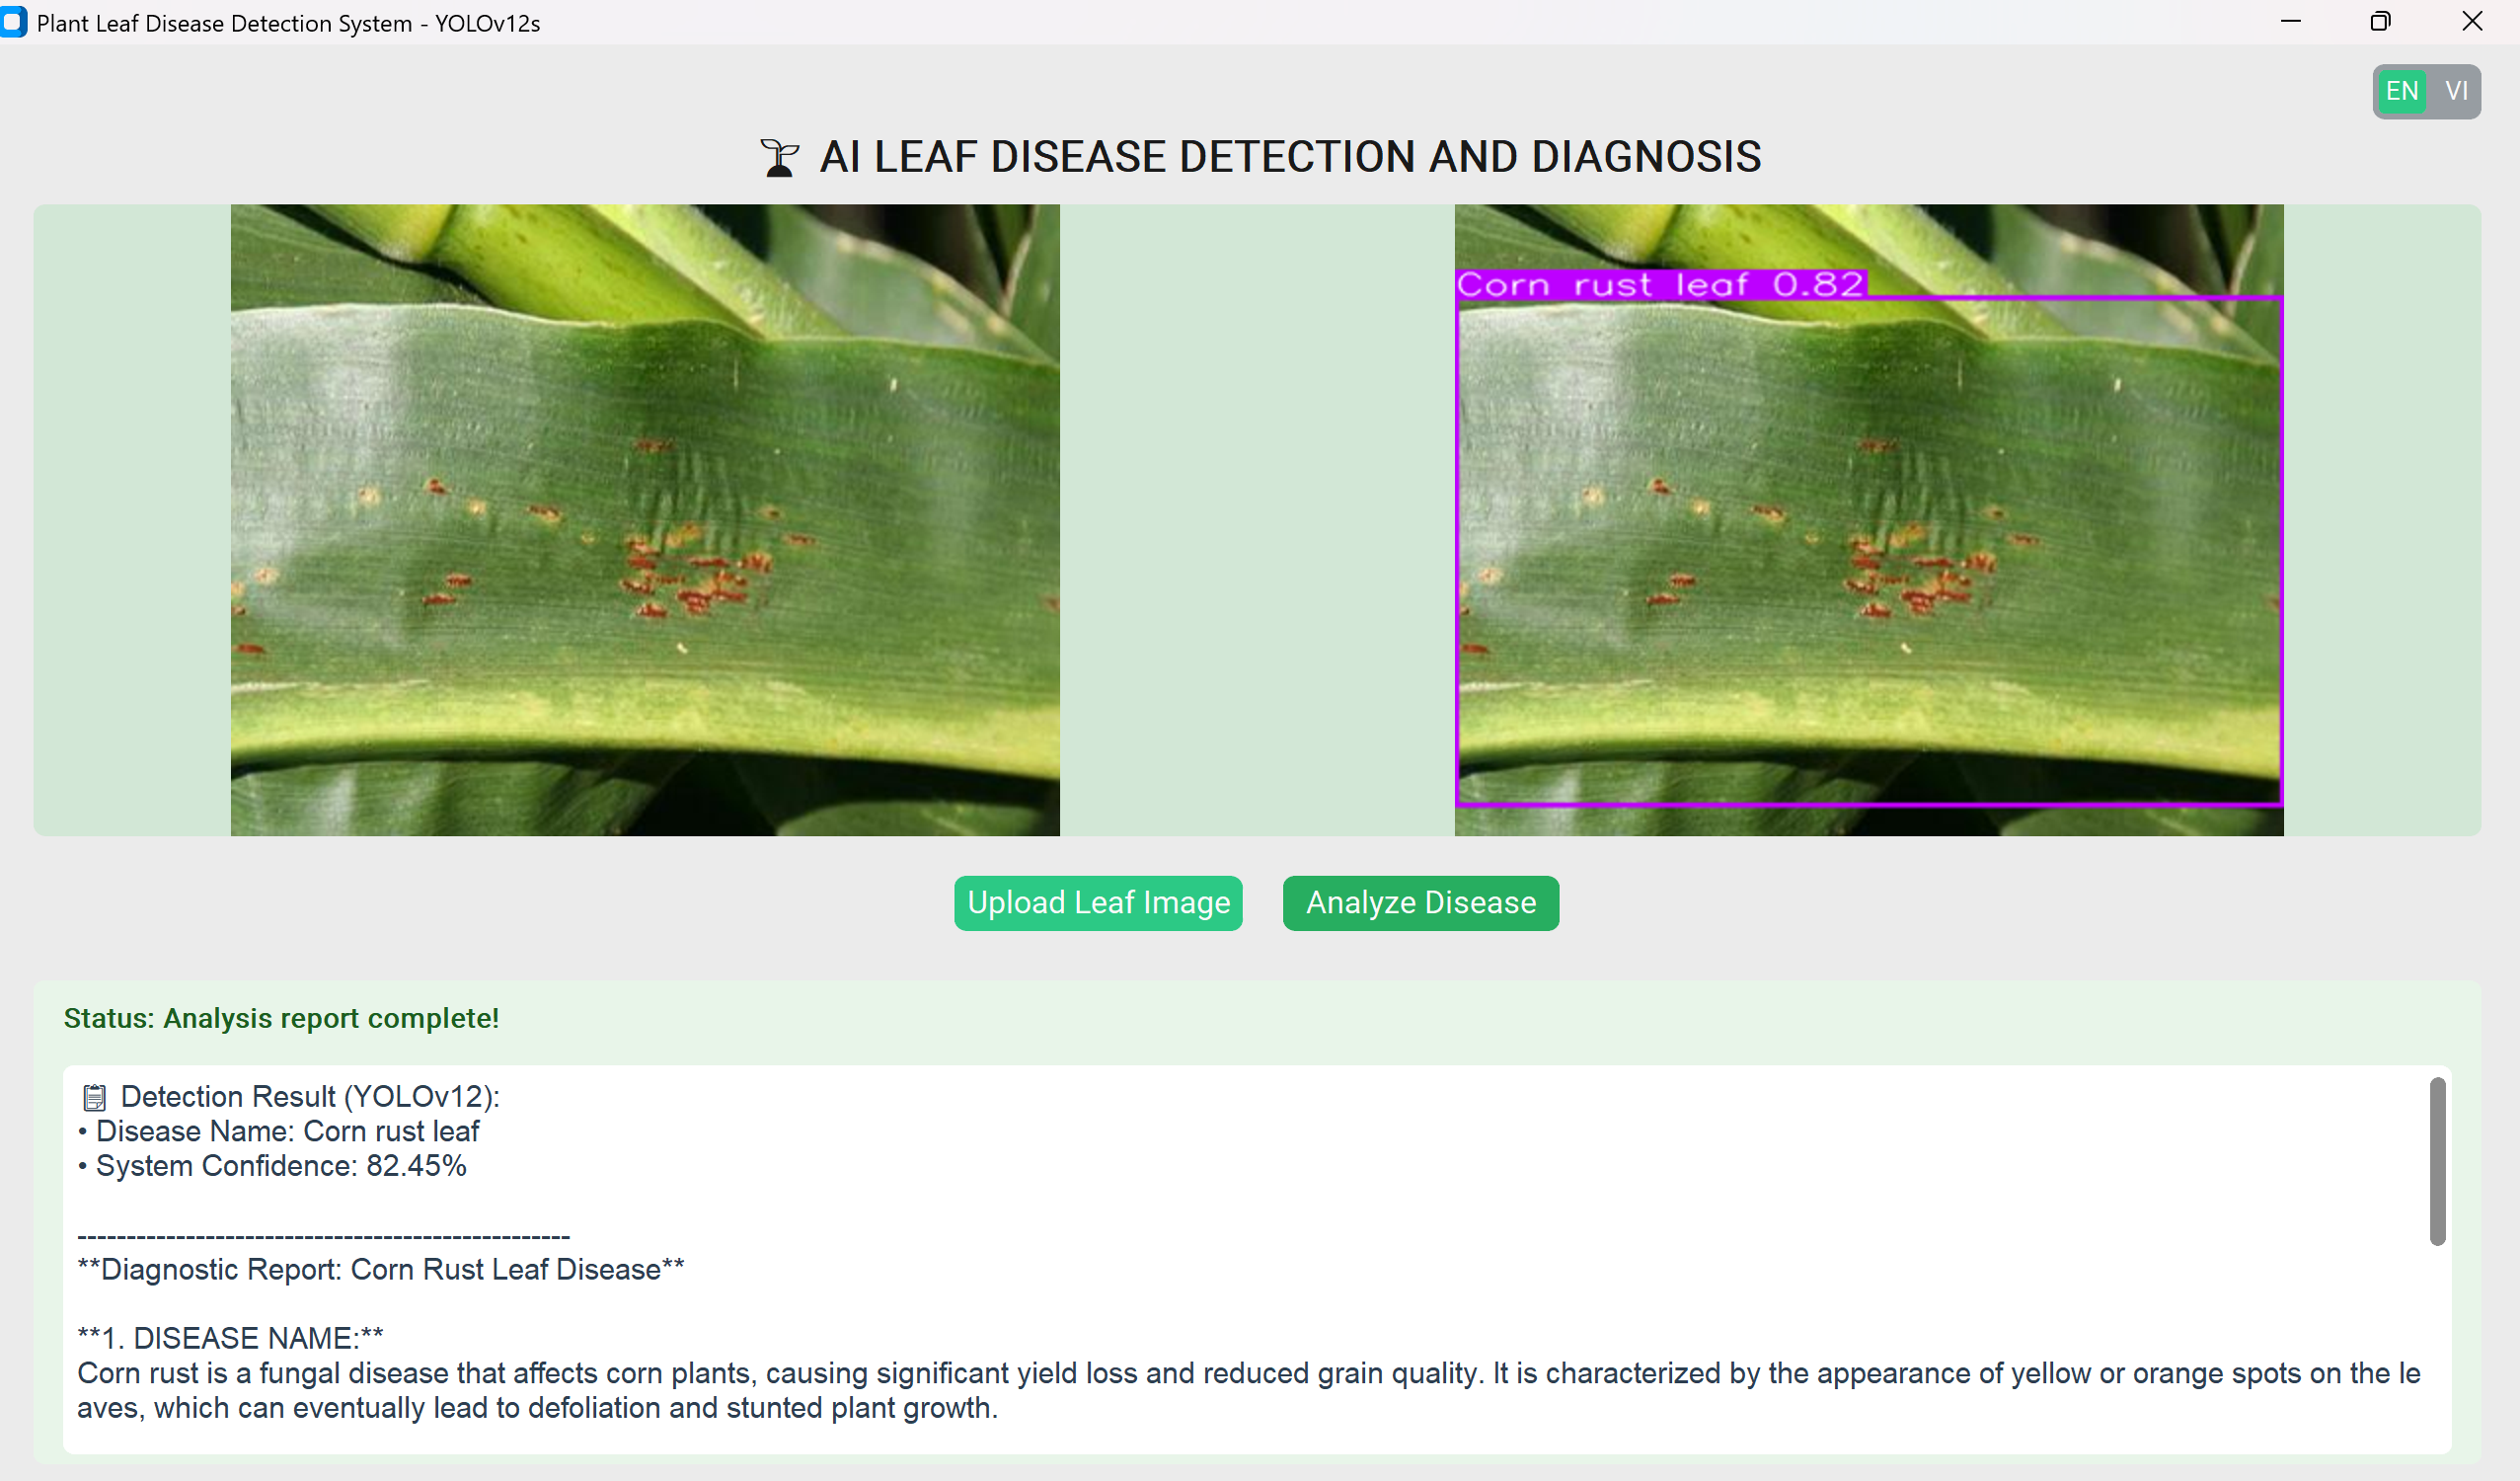
\includegraphics[width=\linewidth]{figures/application.png}
    \caption{Screenshot of the Plant Leaf Disease Detection and Diagnosis application.}
    \label{fig:app}
\end{figure}

%% ============================================================
\balance
\section{Conclusion}
\label{sec:conclusion}

This report has presented the complete pipeline, model architectures, experimental
settings, and results for Group 2's plant leaf disease detection project.
Three state-of-the-art lightweight architectures were implemented and evaluated:
the Advanced Depthwise CNN~\cite{ashurov2025}, V2PlantNet~\cite{nnamdi2025}, and
YOLO-LeafNet~\cite{kaur2025}.

Key findings:
\begin{itemize}
    \item All models achieve near-perfect performance on the controlled PlantVillage
          dataset ($>$98\% accuracy; $>$99\% mAP@50), confirming the viability of
          lightweight architectures.
    \item Performance degrades substantially on the real-world PlantDoc dataset,
          underscoring the importance of training on diverse, field-collected data.
    \item \texttt{WeightedRandomSampler} provides a practical mechanism for
          increasing minority-class exposure, although its isolated effect requires
          an ablation study.
    \item YOLOv12s and YOLOv5s provide the strongest detection accuracy on PlantDoc
          among the evaluated detectors.
\end{itemize}

Future work includes repeated experiments with uncertainty estimates, controlled
ablation studies, train-on-laboratory/test-on-field evaluation, fine-tuning on more
diverse field datasets, and latency measurement on actual edge devices. Knowledge
distillation and model quantisation are also promising directions for reducing
deployment cost.

%% ============================================================
%% Bibliography
%% ============================================================
\bibliographystyle{ieeetr}
%% If using BibTeX, create a references.bib file and uncomment:
%% \bibliography{references}

%% Inline bibliography (fallback if not using BibTeX)
\begin{thebibliography}{99}

\bibitem{harakannanavar2022}
S. S. Harakannanavar, J. M. Rudagi, V. I. Puranikmath, A. Siddiqua, and R. Pramodhini,
``Plant leaf disease detection using computer vision and machine learning algorithms,''
\textit{Global Transitions Proceedings}, vol.~3, no.~1, pp.~305--310, 2022.
\url{https://doi.org/10.1016/j.gltp.2022.03.016}

\bibitem{zhao2025}
J. Zhao, L. Xu, Z. Ma, J. Li, X. Wang, Y. Liu, and X. Du,
``A review of plant leaf disease identification by deep learning algorithms,''
\textit{Front. Plant Sci.}, vol.~16, p.~1637241, 2025.
\url{https://doi.org/10.3389/fpls.2025.1637241}

\bibitem{salka2025}
T. D. Salka, M. B. Hanafi, S. M. S. A. A. Rahman \textit{et al.},
``Plant leaf disease detection and classification using convolution neural networks
model: a review,''
\textit{Artif. Intell. Rev.}, vol.~58, p.~322, 2025.
\url{https://doi.org/10.1007/s10462-025-11234-6}

\bibitem{sujatha2025}
R. Sujatha, S. Krishnan, J. M. Chatterjee \textit{et al.},
``Advancing plant leaf disease detection integrating machine learning and deep
learning,''
\textit{Sci. Rep.}, vol.~15, p.~11552, 2025.
\url{https://doi.org/10.1038/s41598-024-72197-2}

\bibitem{ashurov2025}
A. Y. Ashurov, M. S. A. M. Al-Gaashani, N. A. Samee, R. Alkanhel, G. Atteia,
H. A. Abdallah, and M. Saleh Ali Muthanna,
``Enhancing plant disease detection through deep learning: a Depthwise CNN with
squeeze and excitation integration and residual skip connections,''
\textit{Front. Plant Sci.}, vol.~15, p.~1505857, 2025.
\url{https://doi.org/10.3389/fpls.2024.1505857}

\bibitem{nnamdi2025}
U. V. Nnamdi and V. Abolghasemi,
``Optimised MobileNet for very lightweight and accurate plant leaf disease detection,''
\textit{Sci. Rep.}, vol.~15, no.~1, p.~43690, 2025.
\url{https://doi.org/10.1038/s41598-025-27393-z}

\bibitem{kaur2025}
R. Kaur, U. Mittal, A. Wadhawan \textit{et al.},
``YOLO-LeafNet: a robust deep learning framework for multispecies plant disease
detection with data augmentation,''
\textit{Sci. Rep.}, vol.~15, p.~28513, 2025.
\url{https://doi.org/10.1038/s41598-025-14021-z}

\bibitem{singh2020plantdoc}
D. Singh, N. Jain, P. Jain \textit{et al.},
``PlantDoc: a dataset for visual plant disease detection,''
in \textit{Proc. 7th ACM IKDD CoDS and 25th COMAD}, 2020, pp.~249--253.

\bibitem{hughes2015plantvillage}
D. Hughes and M. Salathé,
``An open access repository of images on plant health to enable the development
of mobile disease diagnostics,''
\textit{arXiv preprint arXiv:1511.08060}, 2015.

\end{thebibliography}

\end{document}
